\documentclass[10pt,journal]{IEEEtran}
%
% If IEEEtran.cls has not been installed into the LaTeX system files,
% manually specify the path to it like:
% \documentclass[10pt,journal,compsoc]{../sty/IEEEtran}





% Some very useful LaTeX packages include:
% (uncomment the ones you want to load)


% *** MISC UTILITY PACKAGES ***
%
%\usepackage{ifpdf}
% Heiko Oberdiek's ifpdf.sty is very useful if you need conditional
% compilation based on whether the output is pdf or dvi.
% usage:
% \ifpdf
%   % pdf code
% \else
%   % dvi code
% \fi
% The latest version of ifpdf.sty can be obtained from:
% http://www.ctan.org/tex-archive/macros/latex/contrib/oberdiek/
% Also, note that IEEEtran.cls V1.7 and later provides a builtin
% \ifCLASSINFOpdf conditional that works the same way.
% When switching from latex to pdflatex and vice-versa, the compiler may
% have to be run twice to clear warning/error messages.






% *** CITATION PACKAGES ***
%
\ifCLASSOPTIONcompsoc
  % IEEE Computer Society needs nocompress option
  % requires cite.sty v4.0 or later (November 2003)
  \usepackage[nocompress,noadjust]{cite}
\else
  % normal IEEE
  \usepackage[noadjust]{cite}
\fi
% cite.sty was written by Donald Arseneau
% V1.6 and later of IEEEtran pre-defines the format of the cite.sty package
% \cite{} output to follow that of IEEE. Loading the cite package will
% result in citation numbers being automatically sorted and properly
% "compressed/ranged". e.g., [1], [9], [2], [7], [5], [6] without using
% cite.sty will become [1], [2], [5]--[7], [9] using cite.sty. cite.sty's
% \cite will automatically add leading space, if needed. Use cite.sty's
% noadjust option (cite.sty V3.8 and later) if you want to turn this off
% such as if a citation ever needs to be enclosed in parenthesis.
% cite.sty is already installed on most LaTeX systems. Be sure and use
% version 5.0 (2009-03-20) and later if using hyperref.sty.
% The latest version can be obtained at:
% http://www.ctan.org/tex-archive/macros/latex/contrib/cite/
% The documentation is contained in the cite.sty file itself.
%
% Note that some packages require special options to format as the Computer
% Society requires. In particular, Computer Society  papers do not use
% compressed citation ranges as is done in typical IEEE papers
% (e.g., [1]-[4]). Instead, they list every citation separately in order
% (e.g., [1], [2], [3], [4]). To get the latter we need to load the cite
% package with the nocompress option which is supported by cite.sty v4.0
% and later. Note also the use of a CLASSOPTION conditional provided by
% IEEEtran.cls V1.7 and later.





% *** GRAPHICS RELATED PACKAGES ***
%
\ifCLASSINFOpdf
  % \usepackage[pdftex]{graphicx}
  % declare the path(s) where your graphic files are
  % \graphicspath{{../pdf/}{../jpeg/}}
  % and their extensions so you won't have to specify these with
  % every instance of \includegraphics
  % \DeclareGraphicsExtensions{.pdf,.jpeg,.png}
\else
  % or other class option (dvipsone, dvipdf, if not using dvips). graphicx
  % will default to the driver specified in the system graphics.cfg if no
  % driver is specified.
  % \usepackage[dvips]{graphicx}
  % declare the path(s) where your graphic files are
  % \graphicspath{{../eps/}}
  % and their extensions so you won't have to specify these with
  % every instance of \includegraphics
  % \DeclareGraphicsExtensions{.eps}
\fi
% graphicx was written by David Carlisle and Sebastian Rahtz. It is
% required if you want graphics, photos, etc. graphicx.sty is already
% installed on most LaTeX systems. The latest version and documentation
% can be obtained at: 
% http://www.ctan.org/tex-archive/macros/latex/required/graphics/
% Another good source of documentation is "Using Imported Graphics in
% LaTeX2e" by Keith Reckdahl which can be found at:
% http://www.ctan.org/tex-archive/info/epslatex/
%
% latex, and pdflatex in dvi mode, support graphics in encapsulated
% postscript (.eps) format. pdflatex in pdf mode supports graphics
% in .pdf, .jpeg, .png and .mps (metapost) formats. Users should ensure
% that all non-photo figures use a vector format (.eps, .pdf, .mps) and
% not a bitmapped formats (.jpeg, .png). IEEE frowns on bitmapped formats
% which can result in "jaggedy"/blurry rendering of lines and letters as
% well as large increases in file sizes.
%
% You can find documentation about the pdfTeX application at:
% http://www.tug.org/applications/pdftex






% *** MATH PACKAGES ***
%
\usepackage[cmex10]{amsmath}
% A popular package from the American Mathematical Society that provides
% many useful and powerful commands for dealing with mathematics. If using
% it, be sure to load this package with the cmex10 option to ensure that
% only type 1 fonts will utilized at all point sizes. Without this option,
% it is possible that some math symbols, particularly those within
% footnotes, will be rendered in bitmap form which will result in a
% document that can not be IEEE Xplore compliant!
%
% Also, note that the amsmath package sets \interdisplaylinepenalty to 10000
% thus preventing page breaks from occurring within multiline equations. Use:
\interdisplaylinepenalty=2500
% after loading amsmath to restore such page breaks as IEEEtran.cls normally
% does. amsmath.sty is already installed on most LaTeX systems. The latest
% version and documentation can be obtained at:
% http://www.ctan.org/tex-archive/macros/latex/required/amslatex/math/





% *** SPECIALIZED LIST PACKAGES ***
%
%\usepackage{algorithmic}
% algorithmic.sty was written by Peter Williams and Rogerio Brito.
% This package provides an algorithmic environment fo describing algorithms.
% You can use the algorithmic environment in-text or within a figure
% environment to provide for a floating algorithm. Do NOT use the algorithm
% floating environment provided by algorithm.sty (by the same authors) or
% algorithm2e.sty (by Christophe Fiorio) as IEEE does not use dedicated
% algorithm float types and packages that provide these will not provide
% correct IEEE style captions. The latest version and documentation of
% algorithmic.sty can be obtained at:
% http://www.ctan.org/tex-archive/macros/latex/contrib/algorithms/
% There is also a support site at:
% http://algorithms.berlios.de/index.html
% Also of interest may be the (relatively newer and more customizable)
% algorithmicx.sty package by Szasz Janos:
% http://www.ctan.org/tex-archive/macros/latex/contrib/algorithmicx/

\usepackage{algpseudocode}


% *** ALIGNMENT PACKAGES ***
%
\usepackage{array}
% Frank Mittelbach's and David Carlisle's array.sty patches and improves
% the standard LaTeX2e array and tabular environments to provide better
% appearance and additional user controls. As the default LaTeX2e table
% generation code is lacking to the point of almost being broken with
% respect to the quality of the end results, all users are strongly
% advised to use an enhanced (at the very least that provided by array.sty)
% set of table tools. array.sty is already installed on most systems. The
% latest version and documentation can be obtained at:
% http://www.ctan.org/tex-archive/macros/latex/required/tools/


% IEEEtran contains the IEEEeqnarray family of commands that can be used to
% generate multiline equations as well as matrices, tables, etc., of high
% quality.




% *** SUBFIGURE PACKAGES ***
\ifCLASSOPTIONcompsoc
  \usepackage[caption=false,font=footnotesize,labelfont=sf,textfont=sf]{subfig}
\else
  \usepackage[caption=false,font=footnotesize]{subfig}
\fi
% subfig.sty, written by Steven Douglas Cochran, is the modern replacement
% for subfigure.sty, the latter of which is no longer maintained and is
% incompatible with some LaTeX packages including fixltx2e. However,
% subfig.sty requires and automatically loads Axel Sommerfeldt's caption.sty
% which will override IEEEtran.cls' handling of captions and this will result
% in non-IEEE style figure/table captions. To prevent this problem, be sure
% and invoke subfig.sty's "caption=false" package option (available since
% subfig.sty version 1.3, 2005/06/28) as this is will preserve IEEEtran.cls
% handling of captions.
% Note that the Computer Society format requires a sans serif font rather
% than the serif font used in traditional IEEE formatting and thus the need
% to invoke different subfig.sty package options depending on whether
% compsoc mode has been enabled.
%
% The latest version and documentation of subfig.sty can be obtained at:
% http://www.ctan.org/tex-archive/macros/latex/contrib/subfig/




% *** FLOAT PACKAGES ***
%
%\usepackage{fixltx2e}
% fixltx2e, the successor to the earlier fix2col.sty, was written by
% Frank Mittelbach and David Carlisle. This package corrects a few problems
% in the LaTeX2e kernel, the most notable of which is that in current
% LaTeX2e releases, the ordering of single and double column floats is not
% guaranteed to be preserved. Thus, an unpatched LaTeX2e can allow a
% single column figure to be placed prior to an earlier double column
% figure. The latest version and documentation can be found at:
% http://www.ctan.org/tex-archive/macros/latex/base/


%\usepackage{stfloats}
% stfloats.sty was written by Sigitas Tolusis. This package gives LaTeX2e
% the ability to do double column floats at the bottom of the page as well
% as the top. (e.g., "\begin{figure*}[!b]" is not normally possible in
% LaTeX2e). It also provides a command:
%\fnbelowfloat
% to enable the placement of footnotes below bottom floats (the standard
% LaTeX2e kernel puts them above bottom floats). This is an invasive package
% which rewrites many portions of the LaTeX2e float routines. It may not work
% with other packages that modify the LaTeX2e float routines. The latest
% version and documentation can be obtained at:
% http://www.ctan.org/tex-archive/macros/latex/contrib/sttools/
% Do not use the stfloats baselinefloat ability as IEEE does not allow
% \baselineskip to stretch. Authors submitting work to the IEEE should note
% that IEEE rarely uses double column equations and that authors should try
% to avoid such use. Do not be tempted to use the cuted.sty or midfloat.sty
% packages (also by Sigitas Tolusis) as IEEE does not format its papers in
% such ways.
% Do not attempt to use stfloats with fixltx2e as they are incompatible.
% Instead, use Morten Hogholm'a dblfloatfix which combines the features
% of both fixltx2e and stfloats:
%
\usepackage{dblfloatfix}
% The latest version can be found at:
% http://www.ctan.org/tex-archive/macros/latex/contrib/dblfloatfix/




%\ifCLASSOPTIONcaptionsoff
%  \usepackage[nomarkers]{endfloat}
% \let\MYoriglatexcaption\caption
% \renewcommand{\caption}[2][\relax]{\MYoriglatexcaption[#2]{#2}}
%\fi
% endfloat.sty was written by James Darrell McCauley, Jeff Goldberg and 
% Axel Sommerfeldt. This package may be useful when used in conjunction with 
% IEEEtran.cls'  captionsoff option. Some IEEE journals/societies require that
% submissions have lists of figures/tables at the end of the paper and that
% figures/tables without any captions are placed on a page by themselves at
% the end of the document. If needed, the draftcls IEEEtran class option or
% \CLASSINPUTbaselinestretch interface can be used to increase the line
% spacing as well. Be sure and use the nomarkers option of endfloat to
% prevent endfloat from "marking" where the figures would have been placed
% in the text. The two hack lines of code above are a slight modification of
% that suggested by in the endfloat docs (section 8.4.1) to ensure that
% the full captions always appear in the list of figures/tables - even if
% the user used the short optional argument of \caption[]{}.
% IEEE papers do not typically make use of \caption[]'s optional argument,
% so this should not be an issue. A similar trick can be used to disable
% captions of packages such as subfig.sty that lack options to turn off
% the subcaptions:
% For subfig.sty:
% \let\MYorigsubfloat\subfloat
% \renewcommand{\subfloat}[2][\relax]{\MYorigsubfloat[]{#2}}
% However, the above trick will not work if both optional arguments of
% the \subfloat command are used. Furthermore, there needs to be a
% description of each subfigure *somewhere* and endfloat does not add
% subfigure captions to its list of figures. Thus, the best approach is to
% avoid the use of subfigure captions (many IEEE journals avoid them anyway)
% and instead reference/explain all the subfigures within the main caption.
% The latest version of endfloat.sty and its documentation can obtained at:
% http://www.ctan.org/tex-archive/macros/latex/contrib/endfloat/
%
% The IEEEtran \ifCLASSOPTIONcaptionsoff conditional can also be used
% later in the document, say, to conditionally put the References on a 
% page by themselves.




% *** PDF, URL AND HYPERLINK PACKAGES ***
%
%\usepackage{url}
% url.sty was written by Donald Arseneau. It provides better support for
% handling and breaking URLs. url.sty is already installed on most LaTeX
% systems. The latest version and documentation can be obtained at:
% http://www.ctan.org/tex-archive/macros/latex/contrib/url/
% Basically, \url{my_url_here}.





% *** Do not adjust lengths that control margins, column widths, etc. ***
% *** Do not use packages that alter fonts (such as pslatex).         ***
% There should be no need to do such things with IEEEtran.cls V1.6 and later.
% (Unless specifically asked to do so by the journal or conference you plan
% to submit to, of course. )

\usepackage{alltt}
\usepackage{tikz}
\usetikzlibrary{arrows.meta}
\usepackage{mathabx}

% for highlighting
\usepackage{color,soul}
\soulregister\cite7
\soulregister\ref7
\soulregister\pageref7


\newcommand{\hide}[1]{\ignorespaces}
\newcommand{\jx}[1]{{\bf Jiaxiang: }#1{ \bf End}}
\newtheorem{theorem}{Theorem}
\newtheorem{lemma}[theorem]{Lemma}
\newtheorem{definition}[theorem]{Definition}

% Define the fontsize in environment {verbatim}
\makeatletter
\def\verbatim{\small\@verbatim \frenchspacing\@vobeyspaces \@xverbatim}
%\def\verbatim@font{\small\ttfamily}
\makeatother


% correct bad hyphenation here
\hyphenation{op-tical net-works semi-conduc-tor}

\usepackage{microtype}


\begin{document}
%
% paper title
% Titles are generally capitalized except for words such as a, an, and, as,
% at, but, by, for, in, nor, of, on, or, the, to and up, which are usually
% not capitalized unless they are the first or last word of the title.
% Linebreaks \\ can be used within to get better formatting as desired.
% Do not put math or special symbols in the title.
\title{Formal Modeling and Verification of a Rate-Monotonic Scheduling Implementation with Real-Time Maude}
%
%
% author names and IEEE memberships
% note positions of commas and nonbreaking spaces ( ~ ) LaTeX will not break
% a structure at a ~ so this keeps an author's name from being broken across
% two lines.
% use \thanks{} to gain access to the first footnote area
% a separate \thanks must be used for each paragraph as LaTeX2e's \thanks
% was not built to handle multiple paragraphs
%
%
%\IEEEcompsocitemizethanks is a special \thanks that produces the bulleted
% lists the Computer Society journals use for "first footnote" author
% affiliations. Use \IEEEcompsocthanksitem which works much like \item
% for each affiliation group. When not in compsoc mode,
% \IEEEcompsocitemizethanks becomes like \thanks and
% \IEEEcompsocthanksitem becomes a line break with idention. This
% facilitates dual compilation, although admittedly the differences in the
% desired content of \author between the different types of papers makes a
% one-size-fits-all approach a daunting prospect. For instance, compsoc 
% journal papers have the author affiliations above the "Manuscript
% received ..."  text while in non-compsoc journals this is reversed. Sigh.

\hide{
\author{Jiaxiang~Liu,
        Min~Zhou,
        Xiaoyu~Song,
        Ming~Gu,
        and~Jiaguang~Sun% <-this % stops a space
\IEEEcompsocitemizethanks{%
\IEEEcompsocthanksitem J. Liu is with the School of Software, Tsinghua
University, Beijing 100084, China, and also with LIX, \'Ecole
Polytechnique, Palaiseau 91120, France.\protect\\ E-mail:
jiaxiang.liu@hotmail.com
\IEEEcompsocthanksitem M. Zhou, M. Gu and J. Sun are with the School
of Software, Tsinghua University, Beijing 100084, China.
\IEEEcompsocthanksitem X. Song is with the Department of Electrical \&
Computer Engineering, Portland State University, Portland, OR
97207-0751, USA.}% <-this % stops an unwanted space
}
%\thanks{Manuscript received April 19, 2005; revised September 17, 2014.}}

% note the % following the last \IEEEmembership and also \thanks - 
% these prevent an unwanted space from occurring between the last author name
% and the end of the author line. i.e., if you had this:
% 
% \author{....lastname \thanks{...} \thanks{...} }
%                     ^------------^------------^----Do not want these spaces!
%
% a space would be appended to the last name and could cause every name on that
% line to be shifted left slightly. This is one of those "LaTeX things". For
% instance, "\textbf{A} \textbf{B}" will typeset as "A B" not "AB". To get
% "AB" then you have to do: "\textbf{A}\textbf{B}"
% \thanks is no different in this regard, so shield the last } of each \thanks
% that ends a line with a % and do not let a space in before the next \thanks.
% Spaces after \IEEEmembership other than the last one are OK (and needed) as
% you are supposed to have spaces between the names. For what it is worth,
% this is a minor point as most people would not even notice if the said evil
% space somehow managed to creep in.
}


% The paper headers
\markboth{IEEE Transaction on xxx,~Vol.~$x$, No.~$x$, xx~$x$}%
{Liu \MakeLowercase{\textit{et al.}}: Formal Modeling and Verification of a Rate-Monotonic Scheduling Implementation with Real-Time Maude}
% The only time the second header will appear is for the odd numbered pages
% after the title page when using the twoside option.
% 
% *** Note that you probably will NOT want to include the author's ***
% *** name in the headers of peer review papers.                   ***
% You can use \ifCLASSOPTIONpeerreview for conditional compilation here if
% you desire.



% The publisher's ID mark at the bottom of the page is less important with
% Computer Society journal papers as those publications place the marks
% outside of the main text columns and, therefore, unlike regular IEEE
% journals, the available text space is not reduced by their presence.
% If you want to put a publisher's ID mark on the page you can do it like
% this:
%\IEEEpubid{0000--0000/00\$00.00~\copyright~2014 IEEE}
% or like this to get the Computer Society new two part style.
%\IEEEpubid{\makebox[\columnwidth]{\hfill 0000--0000/00/\$00.00~\copyright~2014 IEEE}%
%\hspace{\columnsep}\makebox[\columnwidth]{Published by the IEEE Computer Society\hfill}}
% Remember, if you use this you must call \IEEEpubidadjcol in the second
% column for its text to clear the IEEEpubid mark (Computer Society jorunal
% papers don't need this extra clearance.)



% use for special paper notices
%\IEEEspecialpapernotice{(Invited Paper)}

% for Computer Society papers, we must declare the abstract and index terms
% PRIOR to the title within the \IEEEtitleabstractindextext IEEEtran
% command as these need to go into the title area created by \maketitle.
% As a general rule, do not put math, special symbols or citations
% in the abstract or keywords.
\IEEEtitleabstractindextext{%
\begin{abstract}
Rate-Monotonic Scheduling (RMS) is one of the most important real-time
scheduling used in industry. There are a large number of results about
RMS, especially on its schedulability. However, the theoretical
results do not contain enough details to be used directly for an
industrial RMS implementation. On the other hand, the correctness of
such an implementation is of the crucial importance. In this paper, we
analyze a realistic RMS implementation by using Real-Time Maude, a
formal modeling language and analysis tool based on rewriting
logic. Overhead and some details of the hardware are taken into
account in the model. We validate the schedulability and the
correctness of the implementation within key scenarios. The soundness
and the completeness of our approach are substantiated.
\end{abstract}


% Note that keywords are not normally used for peerreview papers.
\begin{IEEEkeywords}
  Real-time systems, scheduling, embedded systems, modeling, formal
  verification, rewriting logic.
\end{IEEEkeywords}
}

% make the title area
\maketitle


% To allow for easy dual compilation without having to reenter the
% abstract/keywords data, the \IEEEtitleabstractindextext text will
% not be used in maketitle, but will appear (i.e., to be "transported")
% here as \IEEEdisplaynontitleabstractindextext when the compsoc 
% or transmag modes are not selected <OR> if conference mode is selected 
% - because all conference papers position the abstract like regular
% papers do.
\IEEEdisplaynontitleabstractindextext
% \IEEEdisplaynontitleabstractindextext has no effect when using
% compsoc or transmag under a non-conference mode.



% For peer review papers, you can put extra information on the cover
% page as needed:
% \ifCLASSOPTIONpeerreview
% \begin{center} \bfseries EDICS Category: 3-BBND \end{center}
% \fi
%
% For peerreview papers, this IEEEtran command inserts a page break and
% creates the second title. It will be ignored for other modes.
\IEEEpeerreviewmaketitle



%\IEEEraisesectionheading{\section{Introduction}\label{s:introduction}}
\section{Introduction}\label{s:introduction}
% Computer Society journal (but not conference!) papers do something unusual
% with the very first section heading (almost always called "Introduction").
% They place it ABOVE the main text! IEEEtran.cls does not automatically do
% this for you, but you can achieve this effect with the provided
% \IEEEraisesectionheading{} command. Note the need to keep any \label that
% is to refer to the section immediately after \section in the above as
% \IEEEraisesectionheading puts \section within a raised box.




% The very first letter is a 2 line initial drop letter followed
% by the rest of the first word in caps (small caps for compsoc).
% 
% form to use if the first word consists of a single letter:
% \IEEEPARstart{A}{demo} file is ....
% 
% form to use if you need the single drop letter followed by
% normal text (unknown if ever used by IEEE):
% \IEEEPARstart{A}{}demo file is ....
% 
% Some journals put the first two words in caps:
% \IEEEPARstart{T}{his demo} file is ....
% 
% Here we have the typical use of a "T" for an initial drop letter
% and "HIS" in caps to complete the first word.
\IEEEPARstart{P}{eriodic} task scheduling is one of the most important
topics within the field of industrial real-time systems.
%due to the large number of control systems that require cyclic activities~\cite{buttazzo2011hard}. 
A set of periodic tasks is said to be \emph{schedulable} with respect
to some scheduling algorithm if all jobs meet their
deadlines. \emph{Rate-Monotonic Scheduling} (\emph{RMS}) is a
\emph{fixed} priority scheduling algorithm for preemptive hard
real-time environments proposed by Liu and
Layland~\cite{DBLP:journals/jacm/LiuL73}, which assigns priorities to
jobs according to the periods of the corresponding tasks: the smaller
period, the higher priority. RMS is proven to be the \emph{optimal}
fixed priority scheduling algorithm~\cite{DBLP:journals/jacm/LiuL73},
in the sense that any set of tasks, which is schedulable under
\emph{some} fixed priority scheduling algorithm, is also schedulable
with respect to RMS. It is widely used in safety-critical real-time
applications, such as vehicles and avionics, thanks to its optimality
and easiness to implement.

Liu and Layland~\cite{DBLP:journals/jacm/LiuL73} gave a sufficient
condition for the schedulability of a set of $n$ tasks scheduled by
RMS: $\displaystyle\Sigma^n_{i=1}C_i/T_i \le n(2^{1/n}-1)$, where
$C_i$ and $T_i$ are the \emph{computation (time) requirement} and the
period of task $\tau_i$, respectively. Two main directions on RMS have
been explored since then. One is to relax the assumptions on the
original RMS model, making it applicable on more systems.  For
instance,
\cite{DBLP:conf/rtss/LehoczkySS87,DBLP:journals/rts/SpruntSL89,DBLP:conf/rtss/LehoczkyR92,DBLP:journals/tc/StrosniderLS95}
allow aperiodic tasks in the scheduling,
\cite{DBLP:journals/pe/LeungW82,audsley1993deadline} generalize RMS to
be \emph{deadline-monotonic}, \cite{DBLP:journals/tc/ShaRL90} allows
resource sharing among tasks,
\cite{dhall1978real,DBLP:journals/rts/LopezGDG03,DBLP:journals/tpds/LopezDG04,DBLP:journals/tc/BaruahG03}
extend RMS on multiprocessors, and
\cite{DBLP:journals/rts/OhS94,DBLP:journals/rts/GhoshMMS98,DBLP:journals/tpds/BertossiMR99}
enhance fault-tolerance. The other direction is to generate better
schedulability test conditions for the algorithm and its
extensions~\cite{DBLP:conf/rtss/LehoczkySD89,DBLP:conf/rtss/KuoM91,DBLP:journals/tc/BiniBB03,DBLP:journals/rts/LopezGDG03,DBLP:journals/tc/BaruahG03,gardner1999}. The
RMS algorithm is no doubt of practical importance.

It is even more crucial to ensure the reliability of an implementation
instead of the algorithm, when RMS serves in a safety-critical
system. When analyzing a realistic implementation, theoretical results
may be no more applicable. For instance, even though the conditions
derived from algorithm analysis are satisfied, schedulability can be
broken by overhead in the system, or by the interrupt mask mechanism
which may delay interrupt handling. On the other hand, correctness of
the implementation with respect to the algorithm is difficult to be
verified by the traditional methods such as testing and simulation due
to their incompleteness. Extensive effort to apply formal methods,
such as model checking and theorem proving, has been made to analyze
safety-critical systems for the past few
years~\cite{DBLP:journals/tie/MiyawakiMSYV05,DBLP:journals/iandc/MeseguerR13,DBLP:journals/cacm/Leroy09,DBLP:conf/sosp/KleinEHACDEEKNSTW09}. However,
as far as we know, few~\cite{DBLP:conf/iceccs/CuiDT14,TianD2011}
attempt to analyze the RMS algorithm, while no work for
implementations of RMS is found.

In this paper, we use \emph{Real-Time Maude}, a \emph{rewriting}-based
formal modeling language and analysis tool for real-time systems, to
model a realistic implementation of RMS that serves as a simplified
operating system within an avionic control system, and then verify
several desired properties. Based on a realistic implementation, our
model extends the standard RMS model proposed
in~\cite{DBLP:journals/jacm/LiuL73}, by considering overhead and other
details of the hardware platform.

The rest of this paper is organized as
follows. Section~\ref{s:background} gives some background of both the
RMS algorithm and Real-Time Maude.  Section~\ref{s:imp} presents the
RMS implementation that we model and analyze.
Section~\ref{s:formalism} introduces how we model the RMS
implementation using Real-Time Maude. Then
Section~\ref{s:verification} explains how to verify the desired
properties and to evaluate the results. Related work is discussed in
Section~\ref{s:relate}. We conclude the paper in
Section~\ref{s:conclusion}.

\section{Background}
\label{s:background}

\subsection{Rate-Monotonic Scheduling Algorithm}
\label{ss:rms}
%\subsection{Formulation of the Standard Setting}
A task set consists of \emph{only} $n$ periodic tasks
$\tau_1,\ldots,\tau_n$. Each task $\tau_i$ has a period $T_i$ and a
computation requirement $C_i$. First jobs of all tasks are assumed to
be initiated at time $0$ simultaneously.  Deadlines consist of
runnability constraints only: the deadline of a job corresponding to
$\tau_i$ is the initiation time of the next job corresponding to
$\tau_i$.  The RMS algorithm chooses the labeling such that $T_1\le
T_2\le \ldots \le T_n$. Consequently, $\tau_i$ receives priority $i$,
assuming smaller numbers have higher priorities. The following
assumptions are made:

(A1) Jobs corresponding to task $\tau_i$ are initiated exactly at
times $kT_i$ with integers $k\ge 0$.

(A2) Computation requirement $C_i$ for each task $\tau_i$ is constant
and does not vary with time.

(A3) Tasks are independent, such that they are ready to run at their
initiation times and can be preempted instantly (ignoring all
blocking).

(A4) All overhead, such as task switching time, is ignored.

A simple example showing this algorithm is depicted in
Figure~\ref{sf:rmsalg}. However in this paper, we consider an
implementation instead of the RMS algorithm itself, thus the model
would be more complicated than this standard, ideal
setting. Assumption~(A1) will be modified because of the interrupt
mask mechanism, while (A4) is relaxed to obtain a more realistic
analysis model.

\subsection{Real-Time Maude}
Real-Time Maude~\cite{DBLP:journals/lisp/OlveczkyM07} is an extension
of \emph{Maude}~\cite{DBLP:journals/tcs/ClavelDELMMQ02} which is a
language and tool based on \emph{rewriting
  logic}~\cite{DBLP:journals/jlp/Meseguer12}.  It supports formal
specification and analysis of real-time systems.

\subsubsection{Specification}
Real-Time Maude models systems as \emph{modules}. A module specifies a
\emph{real-time rewrite theory} ${\cal R} = (\Sigma, E\cup A ,
\mathit{IR}, \mathit{TR})$, where:
\begin{itemize}
\item $\Sigma$ is an algebraic \emph{signature}, that is, a set of
  declarations of \emph{sorts}, \emph{subsorts} and \emph{function
    symbols}. The function symbols are allowed to be mixfix, in which
  case underscores ``\verb|_|'' indicate the positions of parameters.
  \emph{Terms} are expressions built from function symbols and
  variables.
\item $(\Sigma, E\cup A)$ is a \emph{membership equational logic
  theory}, with $E$ a set of \emph{conditional equations} and
  \emph{memberships} on $\Sigma$, and $A$ a set of equational axioms
  such as associativity, commutativity and identity.  $(\Sigma, E\cup
  A)$ models the system's ``static'' states as terms of some sort, and
  is equipped with a built-in specification of a sort \verb|Time|.
\item $\mathit{IR}$ is a set of \emph{labeled conditional rewrite
  rules} specifying the system's local transitions. Each rule has the
  form $[l]~:~t\rightarrow t'\mbox{ \textbf{if}
  }\bigwedge^n_{j=1}cond_j$, where each $cond_j$ is an equality
  $u_j=v_j$, and $l$ is a \emph{label}, \hl{$t,t',u_j,v_j$ are terms}. Such
  a rule specifies an \emph{instantaneous transition}, without
  consuming time, from an instance of $t$ to the corresponding
  instance of $t'$, \emph{provided} the conditions hold.
\item $\mathit{TR}$ is a set of (\emph{labeled}) \emph{tick rules} of
  the form $[l]~:~\{s\}\rightarrow\{s'\} \mbox{\textbf{ in time}
  }r\mbox{ \textbf{if} }cond$ that specify \emph{timed
    transitions}. \hl{Each tick rule advances time by $r$ time units from
  the \emph{entire} state modeled by term $s$ to the destination state
  $s'$.}
\end{itemize}

\hl{$\mathit{IR}$ and $\mathit{TR}$ together model the ``dynamic''
behaviors of the system.}

In rewriting logic, rewrite rules are applied non-deterministically,
that is, when several rules can be applied on a given term $t$, any of
them may be chosen. Hence non-deterministic behaviors can be modeled
naturally in Real-Time Maude.  Real-Time Maude also supports
specifications in \emph{object-oriented} style.  A class declaration
$\texttt{class }C\texttt{ |
}att_1\texttt{:}s_1\texttt{,}\ldots\texttt{,}att_n\texttt{:}s_n$
defines a class $C$ with attributes $att_1$ to $att_n$ of sorts $s_1$
to $s_n$, respectively. An \emph{object} of class $C$ is represented
as a term $\texttt{< } O\texttt{:} C \texttt{ | }
att_1\texttt{:}val_1\texttt{,} \ldots
\texttt{,}att_n\texttt{:}val_n\texttt{ >}$ of sort \verb|Object|,
where $O$, of sort \verb|Oid|, is the object's \emph{identifier}, and
$val_i$ is the value of the attribute $att_i$ with $i\in [1,n]$. Rules
can be defined on a given class. A \emph{subclass} inherits all the
attributes and rules of its superclasses.

\subsubsection{Formal Analysis}
Real-Time Maude provides many useful commands and tools to analyze a
given model. For example, \verb|rewrite| allows to execute the model,
symbolically; given an initial state, \verb|search| is used to search
reachable states satisfying the desired properties; the Maude's
\emph{Inductive Theorem Prover} (ITP) can be applied to interactively
prove properties written in \emph{membership equational logic}.

In this paper, we only consider Real-Time Maude's \emph{Linear
  Temporal Logic (LTL) model checker}, which analyzes whether
\emph{each} behavior satisfies a temporal logic formula. \emph{State
  propositions} are defined as terms of sort \verb|Prop|. Their
semantics is defined by conditional equations of the form $\texttt{ceq
} statePattern \texttt{ |= } prop \texttt{ = } b \texttt{ if } cond$,
with $b$ a term of sort \verb|Bool|, stating that $prop$ evaluates to
$b$ in states which are instances of $statePattern$ provided the
condition $cond$ holds. These equations together define $prop$ to hold
in all states $s$ that make $s \texttt{ |= } prop$ evaluate to
\verb|true|. A temporal logic \emph{formula} is constructed by state
propositions and \hl{temporal logic operators such as} \verb|~|\hl{(negation),}
\verb|\/|\hl{(disjunction),} \verb|[]|\hl{(``always''),}
\verb|U|\hl{(``until'')}. Real-Time Maude supports both \emph{timed} and
\emph{untimed LTL model checking}. The untimed model checking command
\begin{alltt}
  (mc \(s\) |=u \(\Phi\) .)
\end{alltt}
checks whether the temporal logic formula $\Phi$ holds in all
behaviors starting from the initial state $s$, \emph{with no time
  limit}.


\section{The Implementation of RMS}
\label{s:imp}
The implementation written in C is from an industrial avionic control
system.  Interrupts would be triggered by, and only by, the clock
every $T$, which we call \emph{interrupt cycle}. When an interrupt
request occurs, if the system is interruptible, i.e. the interrupt
mask bit is cleared, the handler function $schedule()$ will be
invoked; otherwise $schedule()$ will be pending until the interrupt
mask bit becomes cleared.  The pseudocode of $schedule()$ is shown in
Figure~\ref{a:schedule}, where $taskList$ is the list of periodic
tasks to be scheduled. We assume that the list is in descending order
of priority, and both variables $taskList$ and $timer$ are global. In
this implementation, there is only one kind of interrupt, the period
$T_i$ of each task is a multiple of $T$, and the tasks are
independent, meeting assumption~(A3).

\begin{figure}[!t]
\hrule\vspace{1mm}
  \begin{algorithmic}[1]\small
\Function{$schedule$}{$ $}{}
  \State \Call{$int\_o\!f\!\!f$}{$ $}; \Comment{to disable interrupts} \label{l:1stline}
  \State \Call{$updateStatus$}{$taskList$}; \label{l:updatestatus}
  \State $timer = timer + 1$; \label{l:timer} \label{l:inc}
  \State $p = taskList$;
  \While{$p$} \label{l:startrun1st}
    \If{$p\rightarrow status == \textit{INTERRUPT}$}
      \State \Return; \label{l:return}
    \ElsIf{$p\rightarrow status == \textit{READY}$}      
      \State $p\rightarrow status = \textit{RUNNING}$;
      \State \Call{$int\_on$}{$ $}; \Comment{to enable interrupts} \label{l:endrun1st}
      \State $p\rightarrow function()$; \Comment{to execute the task} \label{l:function}
      \State \Call{$int\_o\!f\!\!f$}{$ $};
      \State $p\rightarrow status = \textit{DORMANT}$;
    \EndIf
    \State $p = p\rightarrow next$;
  \EndWhile
\EndFunction
\Function{$updateStatus$}{$p$}
  \While{$p$}
    \If{$p\rightarrow status == \textit{RUNNING}$} \label{l:startupdate}
      \State $p\rightarrow status = \textit{INTERRUPT}$;
    \EndIf
    \If{$timer~\%~(p\rightarrow period) == 0$} \Comment{the task should be initiated}
      \If{$p\rightarrow status == \textit{DORMANT}$} \Comment{the previous job finishes} 
        \State $p\rightarrow status = \textit{READY}$;
      \Else \Comment{the status is \textit{READY} or \textit{INTERRUPT}}
  \State \Call{$reportTaskError$}{$p$}; \Comment{task misses its deadline}
      \EndIf
    \EndIf \label{l:endupdate}
    \State $p = p\rightarrow next$;
  \EndWhile
\EndFunction
  \end{algorithmic}
\hrule
  \caption{The C-Like Pseudo-code of $schedule()$}
  \label{a:schedule}
\end{figure}

In Figure~\ref{a:schedule}, the handler function $schedule()$ first
updates status of all tasks in $taskList$ via function
$updateStatus()$. This updating actually initiates tasks that should
be scheduled in the current interrupt cycle. Then $schedule()$
traverses the list to execute the ready tasks one by one, or to do a
return when encountering an interrupted\footnote{Note that the status
  \textit{INTERRUPT} indicates the task is interrupted for the moment,
  or was interrupted before but its execution is not complete yet.}
task. As for the function $updateStatus()$, it updates each task in
two steps: firstly, if the task is running, it becomes interrupted;
secondly for the task at its initiation time, if its previous job is
complete, it would be set ready, otherwise it misses its deadline,
producing an error. Notice that $schedule()$ is invoked only when the
interrupt request is handled, not when the interrupt is disabled (the
interrupt mask bit is set). Due to the interrupt mask bit, its
execution cannot be interrupted when it is updating status of tasks or
searching the next task to execute, however, it can be interrupted
while executing some task (Line~\ref{l:function}). This allows the
execution of $schedule()$ to be nested.

For simplicity, in the rest of this paper, we use \emph{scheduling} to
refer to the stage, from the moment when a pending interrupt request
is detected, to the moment when the first should-be-run periodic task
starts executing, i.e. Line~\ref{l:return} or~\ref{l:function} in
Figure~\ref{a:schedule}. Therefore, \emph{scheduling time} mainly
consists of three parts: (i) the time for switching context from the
running task, possibly none, to $schedule()$ when an interrupt request
is handled, (ii) the time spent by $schedule()$ searching and setting
the \emph{first} should-be-run periodic task
(Lines~\ref{l:1stline}-\ref{l:endrun1st} in Figure~\ref{a:schedule}),
and (iii) the time for switching context from $schedule()$ to that
task. \emph{Switching} refers to the stage, from the moment when a
periodic task completes its execution, to the moment when the next
should-be-run periodic task starts executing. \emph{Switching time}
thus also consists of three parts: (i) the time for switching context
from the complete task back to $schedule()$, (ii) the time spent by
$schedule()$ searching and setting the \emph{next} should-be-run
periodic task, and (iii) the time for switching context from
$schedule()$ to that task.


\section{Formal Modeling of the Implementation}
\label{s:formalism}
Considering some technical details of the platform, such as interrupt
mask mechanism, we model the implementation under the following
assumptions:

(A1') Jobs corresponding to task $\tau_i$ are initiated at the
beginning of scheduling that handles the requests triggered at times
$kT_i$ with integers $k\ge 0$.

(A2) Computation requirement $C_i$ for each task $\tau_i$ is constant
and does not vary with time.

(A3) Tasks are independent, such that they are ready to run at their
initiation times and can be preempted instantly.

(A4') Scheduling time and switching time are considered, while other
overhead is ignored.

These assumptions make our model different from the standard one. For
instance, with assumption~(A1'), an interrupt request that occurs
during switching will be pending, such that jobs of task $\tau_i$
cannot initiate at $kT_i$. They should wait until switching finishes
and the interrupt mask bit is cleared, which is different
from~(A1). Note that (A3) says that jobs are ready to run at their
initiation times, however, no one can start running at exactly its
initiation time, because scheduling takes time. Under these
assumptions, an example showing the execution of tasks scheduled by
the implementation is depicted in Figure~\ref{sf:rmsimp}. Note that
the second job instance of $\tau_1$ is initiated at time $11$ instead
of $10$, because switching is performed and the interrupt mask bit is
set at time $10$, exemplifying differences between (A1') and (A1).

\begin{figure}[!t]
\centering
\subfloat[RMS Algorithm]{
  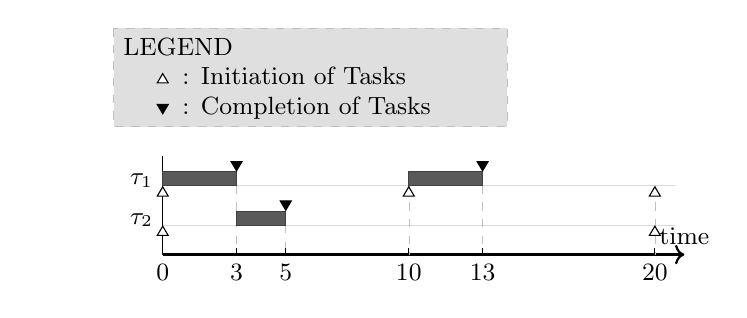
\begin{tikzpicture}[font=\small,scale=1.25,
    % styles
    system task/.style={fill=gray!70,draw=gray},
    periodic task/.style={fill=gray!70!black,draw=gray!50!black},
    task line/.style={gray!30,very thin},
    time line/.style={gray!50,very thin,dashed},
    short line/.style={gray!50,very thin,dashed},
    init/.style={{Triangle[fill=white,scale=1.1]}-},
    complete/.style={{Triangle[scale=1.1]}-}]

  % legend
  \begin{scope}[xshift=-2cm]  
    \draw [fill=gray!25,draw=gray!50,dashed] (1.5,2.3) rectangle +(4,-1);
    \draw (1.5,2.3) node [below right] {LEGEND};
    \draw [init] (2,1.85) -- +(0,-0.01);
    \draw (2.1,2) node [below right] {: Initiation of Tasks};
    \draw [complete] (2,1.42) -- +(0,0.1);
    \draw (2.1,1.7) node [below right] {: Completion of Tasks};
  \end{scope}
  
    % grid
    \foreach \x in {0.3,0.7}
      \draw[task line] (0,\x) -- (5.2,\x);

    % axes
    \draw[->,thick] (0,0) node [below] {$0$} -- (5.3,0) node [above] {time};
    \draw[thin] (0,0) -- (0,1);

    % time indicator
    \draw [time line] (0.75,0.7) -- (0.75,0);
    \draw (0.75,0) node [below] {$3$} -- +(0,2pt);
    \draw [time line] (1.25,0.3) -- (1.25,0);
    \draw (1.25,0) node [below] {$5$} -- +(0,2pt);
    \draw [time line] (2.5,0.7) -- (2.5,0);
    \draw (2.5,0) node [below] {$10$} -- +(0,2pt);
    \draw [time line] (3.25,0.7) -- (3.25,0);
    \draw (3.25,0) node [below] {$13$} -- +(0,2pt);

    \draw [time line] (5,0.7) -- (5,0);
    \draw (5,0) node [below] {$20$} -- +(0,2pt);
    
    % tasks
    \draw [periodic task] (0,0.7) rectangle +(0.75,0.14);
    \draw [periodic task] (0.75,0.3) rectangle +(0.5,0.14);
    \draw [periodic task] (2.5,0.7) rectangle +(0.75,0.14);

    % text
    \draw (0,0.75) node [left] {$\tau_1$};
    \draw (0,0.35) node [left] {$\tau_2$};
    \path (0,0.75) node [left,text opacity=0] {scheduling};
    \path (0,0.35) node [left,text opacity=0] {switching};    

    % initiation of tasks
    \foreach \x in {0,2.5,5}
      \draw [init] (\x,0.7) -- +(0,-0.01);
    \foreach \x in {0,5}
      \draw [init] (\x,0.3) -- +(0,-0.01);  

    % completion of tasks
    \draw [complete] (0.75,0.84) -- +(0,0.01);
    \draw [complete] (3.25,0.84) -- +(0,0.01);
    \draw [complete] (1.25,0.44) -- +(0,0.01);
  \end{tikzpicture}
\label{sf:rmsalg}}\\
\subfloat[RMS Implementation]{
  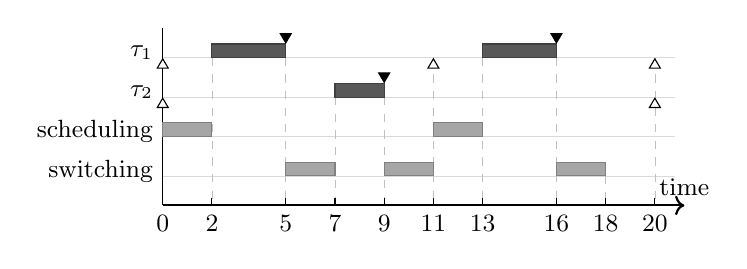
\begin{tikzpicture}[font=\small,scale=1.25,
    % styles
    system task/.style={fill=gray!70,draw=gray},
    periodic task/.style={fill=gray!70!black,draw=gray!50!black},
    task line/.style={gray!30,very thin},
    time line/.style={gray!50,very thin,dashed},
    short line/.style={gray!50,very thin,dashed},
    init/.style={{Triangle[fill=white,scale=1.1]}-},
    complete/.style={{Triangle[scale=1.1]}-}]

    % grid
    \foreach \x in {0.3,0.7,1.1,1.5}
      \draw[task line] (0,\x) -- (5.2,\x);

    % axes
    \draw[->,thick] (0,0) node [below] {$0$} -- (5.3,0) node [above] {time};
    \draw[thin] (0,0) -- (0,1.8);

    % time indicator
    \draw [time line] (0.5,1.5) -- (0.5,0);
    \draw (0.5,0) node [below] {$2$} -- +(0,2pt);
    \draw [time line] (1.25,1.5) -- (1.25,0);
    \draw (1.25,0) node [below] {$5$} -- +(0,2pt);
    \draw [time line] (1.75,1.1) -- (1.75,0);
    \draw (1.75,0) node [below] {$7$} -- +(0,2pt);
    \draw [time line] (2.25,1.1) -- (2.25,0);
    \draw (2.25,0) node [below] {$9$} -- +(0,2pt);
    \draw [time line] (2.75,1.5) -- (2.75,0);
    \draw (2.75,0) node [below] {$11$} -- +(0,2pt);
    \draw [time line] (3.25,1.5) -- (3.25,0);
    \draw (3.25,0) node [below] {$13$} -- +(0,2pt);
    \draw [time line] (4,1.5) -- (4,0);
    \draw (4,0) node [below] {$16$} -- +(0,2pt);
    \draw [time line] (4.5,0.3) -- (4.5,0);
    \draw (4.5,0) -- +(0,2pt);
    \draw (4.5,0) node [below] {$18$};
    \draw [time line] (5,1.5) -- (5,0);
    \draw (5,0) node [below] {$20$} -- +(0,2pt);
    
    % tasks
    \draw [system task] (0,0.7) rectangle +(0.5,0.14);
    \draw [periodic task] (0.5,1.5) rectangle +(0.75,0.14);
    \draw [system task] (1.25,0.3) rectangle +(0.5,0.14);
    \draw [periodic task] (1.75,1.1) rectangle +(0.5,0.14);
    \draw [system task] (2.25,0.3) rectangle +(0.5,0.14);
    \draw [system task] (2.75,0.7) rectangle +(0.5,0.14);
    \draw [periodic task] (3.25,1.5) rectangle +(0.75,0.14);
    \draw [system task] (4,0.3) rectangle +(0.5,0.14);

    % text
    \draw (0,1.55) node [left] {$\tau_1$};
    \draw (0,1.15) node [left] {$\tau_2$};
    \draw (0,0.75) node [left] {scheduling};
    \draw (0,0.35) node [left] {switching};    

    % initiation of tasks
    \foreach \x in {0,2.75,5}
      \draw [init] (\x,1.5) -- +(0,-0.01);
    \foreach \x in {0,5}
      \draw [init] (\x,1.1) -- +(0,-0.01);  

    % completion of tasks
    \draw [complete] (1.25,1.64) -- +(0,0.01);
    \draw [complete] (2.25,1.24) -- +(0,0.01);
    \draw [complete] (4,1.64) -- +(0,0.01);
  \end{tikzpicture}
\label{sf:rmsimp}}
\caption{A set of $2$ periodic tasks scheduled under RMS algorithm and
  the implementation, respectively. $T=T_1=10$, $T_2=20$, $C_1=3$,
  $C_2=2$. In Figure~\ref{sf:rmsimp}, we assume both scheduling time
  and switching time are $2$.}
\label{f:example}
\end{figure}

In this section, we introduce first how we model the states--the
static aspect--of the system using terms of given sorts, or called
data types, then how we specify the essential behaviors--the dynamic
aspect--using rewrite rules. In particular, modeling of
\emph{instantaneous behaviors} would be explained in
Sections~\ref{ss:ir}, \ref{ss:init} and~\ref{ss:inthandling}, followed
by \emph{timed behaviors} in Section~\ref{ss:timedbehavior}.

\subsection{Basic Data Types}
In our model, tasks are identified by their indexes of sort \verb|Nat|
in the $taskList$. We define a sort \verb|MaybeNat| wrapping
\verb|Nat|s to refer to some task, with \emph{constructor} \verb|some|
followed by a \verb|Nat| $n$ indicating the task indexed $n$, and
\verb|none| for no task:
\begin{verbatim}
  op none : -> MaybeNat [ctor] .
  op some_ : Nat -> MaybeNat [ctor] .
\end{verbatim}
where the keyword \verb|ctor| denotes the corresponding function
symbol to be a constructor.

A sort \verb|Stack| is introduced to model the stack of the system,
storing the tasks that are being interrupted, and equipped with
operations \verb|push|, \verb|pop| and \verb|peek| on it.
\hide{
\begin{verbatim}
  op bottom : -> Stack [ctor] .
  op _#_ : Nat Stack -> Stack [ctor] .
\end{verbatim}
}

We also need
%a sort \verb|Interval| to denote computation requirements of tasks, and 
a sort \verb|Counter| to record the execution of tasks.  We call
\emph{execution time} the time how long a task has been executing
for. A \verb|Counter| records the execution time and the computation
requirement of a task.
\hide{
\begin{verbatim}
  op [_/_] : Time Time -> Counter [ctor] .
\end{verbatim}
}

\hide{
At last, to make our model checkable by untimed model checking, it is
reasonable to reset the global variable $timer$ when it reaches an
upper bound while increasing (see Line~\ref{l:timer} in
Figure~\ref{a:schedule}) in the model. Then $timer$ is of sort
\verb|Timer| and the upper bound would be the least common multiple of
the periods of all tasks.}

The global variable $timer$ is reset when it reaches an upper bound
while increasing, which is not shown in detail in
Figure~\ref{a:schedule} but is reasonable. The upper bound is the
least common multiple of the periods of all tasks. A sort \verb|Timer|
is defined to model the $timer$.
\hide{
\begin{verbatim}
  op [_/_] : Nat NzNat -> Timer [ctor] .
\end{verbatim}
}

\subsection{Modeling the System States}
The system can be considered as consisting of several parts: the tasks
which are scheduled, the scheduler itself, the hardware including
registers and stacks, and the interrupt source. The scheduler,
i.e. the function $schedule()$, can be described by a single variable
$timer$. We present the models of the other parts one by one.

\subsubsection{Tasks}
Each task is abstracted from its functionality as a \verb|Counter|.
Overhead for scheduling and switching is considered in our model. They
are treated as two system tasks. Every task is modeled as an object
instance of some subclass of the base class \verb|Task|:
\begin{verbatim}
  class Task | cnt : Counter .
  op error : -> Object [ctor] .
\end{verbatim}
where \verb|error| is an object indicating some task that misses its
deadline.

A periodic task, which needs to be scheduled, is an object instance of
the subclass \verb|PTask| of \verb|Task| with additional attributes
\verb|priority|, \verb|period| and \verb|status|:
%  class PTask | priority : Nat, period : NzNat, 
\begin{verbatim}
  class PTask | priority : Nat, period : Nat, 
                status : Status .
  subclass PTask < Task .
\end{verbatim}
where \verb|Status| is a sort with four constant constructors
\verb|RUNNING|, \verb|INTERRUPT|, \verb|READY| and \verb|DORMANT|,
same as in the implementation.
\hide{
\begin{verbatim}
  ops RUNNING INTERRUPT READY DORMANT 
        : -> Status [ctor] .
\end{verbatim}
} 

The list of periodic tasks, the variable $taskList$ in the
implementation, is modeled as an instance of sort \verb|TaskList|,
which is a list of \verb|PTask|s and/or \verb|error|s.
\hide{
\begin{verbatim}
  op null : -> TaskList [ctor] .
  op _::_ : Object TaskList 
              ~> TaskList [ctor] .
  mb (< O:Oid : PTask |> :: L:TaskList) 
       : TaskList .
  mb (error :: L:TaskList) : TaskList .
\end{verbatim}
}
Periodic tasks are identified by their indexes in the list.

On the other hand, a system task is an object instance of the subclass
\verb|SysTask| of \verb|Task| with no extra attributes:
\begin{verbatim}
  class SysTask | .  
  subclass SysTask < Task .
\end{verbatim}
Different from periodic tasks, system tasks are organized in a
multiset of sort \verb|SysTasks|, and identified by their \verb|Oid|s.
%We abstract here from the detailed definitions thanks to the
%similarity.

\subsubsection{Hardware}
Our model considers two parts of hardware related to the interrupt
handling mechanism: the registers and the stack.

The set of registers is modeled as an object instance of the class
\verb|Regs|, with attributes \verb|pc| denoting the program counter,
\verb|mask| for the interrupt mask bit and \verb|ir| for the interrupt
request bit, respectively:
\begin{verbatim}
  class Regs | pc : TaskID, 
               mask : Bool, ir : Bool .
\end{verbatim}
where the sort \verb|TaskID| contains subsorts \verb|MaybeNat| and
\verb|Oid|, referring to some task.
\hide{
\begin{verbatim}
  subsorts MaybeNat Oid < TaskID .
\end{verbatim}
}
Some operations, such as \verb|getPc| and \verb|setMask|, are defined
on the class \verb|Regs|.

Then the hardware is described by the sort \verb|Hardware| consisting
of an instance of \verb|Regs| and a term of sort \verb|Stack|.  
\hide{
\begin{verbatim}
  op [_;_] : Object Stack ~> Hardware [ctor] .
  mb ([ < O:Oid : Regs |> ; S:Stack ]) 
       : Hardware .
\end{verbatim}
}

\subsubsection{Interrupt Source}
The interrupt source is modeled as an object of class \verb|IntSrc|,
with attributes \verb|cycle| denoting the interrupt cycle $T$, and
\verb|val| for the value which will decrease from $T$ to $0$ while
time advances:
\begin{verbatim}
  class IntSrc | val : Time, cycle : Time .
\end{verbatim}

\subsubsection{System}
The entire system in our model is a composition of the parts
introduced above, of a sort \verb|System|\footnote{Following the Maude
  convention, variables would be written in capital letters. Some
  variable declarations are not shown for simplicity.}:
\begin{verbatim}
  op _____ : TaskList Timer SysTasks 
             Hardware Object ~> System [ctor] .
  mb (L T STS HW < O : IntSrc |>) : System .
\end{verbatim}
where ``\verb|~>|'' means that the function defined is a partial
function and the keyword \verb|mb| declares a membership axiom,
stating here that a term composed of a \verb|TaskList|, a
\verb|Timer|, a \verb|SysTasks|, a \verb|Hardware| and an object
instance of class \verb|IntSrc| is of sort \verb|System|.

\subsection{Interrupt Requests}
\label{ss:ir}
Interrupt requests are performed by the source exactly every cycle
$T$, when the attribute \verb|val| decreases to \verb|zero|. The
requesting is an instantaneous action, thus is modeled by the
following instantaneous conditional rule applied on \verb|System|:
\begin{verbatim}
  crl [interrupt-request] :
    (L T STS HW ISRC) 
    => (L T STS (HW).intReq reset(ISRC))
    if (ISRC).timeout .
\end{verbatim}
where the function \verb|_.timeout| examines whether the attribute
\verb|val| equals \verb|zero|, and \verb|_.intReq| sets the \verb|ir|
bit indicating there exists an interrupt request to be handled.
\hide{
\begin{verbatim}
  op _.intReq : Hardware -> Hardware .
  eq [ REGS ; S ].intReq 
       = [ (REGS).setIr ; S ] .
\end{verbatim}
}

Then the request will wait to be handled, which is explained in
Section~\ref{ss:inthandling}.

\subsection{Task Initiation}
\label{ss:init}
Periodic tasks are initiated sequentially by the function
$updateStatus()$ in Figure~\ref{a:schedule}, which is treated as an
instantaneous action in our model. It is modeled by a recursive
function \verb|updateStatus_with_|:
\begin{verbatim}
  op updateStatus_with_ : TaskList Timer 
                            -> TaskList . 
\end{verbatim}
%  eq updateStatus null with TIMER = null .
%  eq updateStatus (TASK :: L) with TIMER
%     = (update TASK with TIMER) 
%       :: (updateStatus L with TIMER) .
which applies function \verb|update_with_| on individual task
sequentially to update the status
(Lines~\ref{l:startupdate}-\ref{l:endupdate} in
Figure~\ref{a:schedule}):
\begin{verbatim}
  op update_with_ : Object Timer ~> Object .
  ceq update < O : PTask | period : T, 
                           status : ST > 
        with TIMER
      = if ST == DORMANT 
        then < O : PTask | status : READY >
        else error fi
      if TIMER rem T == 0 .
  eq update < O : PTask | status : ST > 
       with TIMER
     = if ST == RUNNING 
       then < O : PTask | status : INTERRUPT >
       else < O : PTask |> fi [otherwise] .
\end{verbatim}
with \verb|TIMER| the current value of the global variable $timer$.
Given a task, if \verb|TIMER|($timer$) can be divided by its period
\verb|T|, this task should be initiated.  In the case where the task
should be initiated, it is set \verb|READY| if its \verb|status| is
\verb|DORMANT|; otherwise that means the previous job of this task is
not complete, hence it misses its deadline, producing an
\verb|error|. In the other case where the task should not be
initiated, its \verb|status| changes only if it is \verb|RUNNING|.

We can see that \verb|updateStatus_with_| behaves the same as
$updateStatus()$ in Figure~\ref{a:schedule}.

\subsection{Interrupt Handling and Task Scheduling}
\label{ss:inthandling}
When an interrupt request occurs, it may not be detected immediately
by the system. It requires the bit \verb|mask| to be cleared. Once the
request is detected, it is handled in two steps: the interrupt
handling mechanism of the hardware (such as clearing \verb|ir|,
pushing context into stack and so on), and to invoke the function
$schedule()$. This behavior is modeled by the following instantaneous
rewrite rule:
\begin{verbatim}
  crl [interrupt-handle] :
    SYSTEM 
    => ((SYSTEM).interrupt).startScheduling
    if (SYSTEM).existInt .
\end{verbatim}
where \verb|_.existInt| checks whether \verb|mask| is cleared
\emph{and} \verb|ir| is set. The function \verb|_.interrupt| models
the interrupt handling mechanism performed by the hardware and does
four things: (i) clearing the bit \verb|ir|, which means the request
has been handled; (ii) pushing the current \verb|pc| into the stack,
storing the interrupted context; (iii) assigning \verb|scheduling| of
sort \verb|Oid| to \verb|pc|, which indicates that the system is
scheduling; and (iv) setting the bit \verb|mask|, to mask coming
interrupt requests.

Unlike periodic tasks, even though the scheduling stage is modeled by
a \verb|Counter|, its functionality is too important to be abandoned.
We divide the behaviors of scheduling into three parts.  The first
part contains its timed behaviors. This part is modeled by regarding
scheduling as a system task of sort \verb|SysTask|. Modeling timed
behaviors of tasks is explained in Section~\ref{ss:timedbehavior}.
The other two parts together define its functionality. The second part
corresponds to Lines~\ref{l:updatestatus}-\ref{l:inc} in
Figure~\ref{a:schedule}. It updates the status of $taskList$ and
increases $timer$ by $1$. This part is modeled by function
\verb|_.startScheduling| which applies instantaneously at the
beginning of scheduling, as shown in rule \verb|interrupt-handle|:
\begin{verbatim}
  op _.startScheduling : System -> System .
  eq (L T STS HW ISRC).startScheduling 
     = ((updateStatus L with T) 
        inc(T) STS HW ISRC) .
\end{verbatim}
The third part corresponds to
Lines~\ref{l:startrun1st}-\ref{l:endrun1st}, searching the first
should-be-run periodic task and setting it to execute. It is modeled
by function \verb|_.finishScheduling|, which applies instantaneously
at the end of scheduling:
\begin{verbatim}
  op _.finishScheduling : System -> System .
  eq (L T STS HW ISRC).finishScheduling
     = (L T (finish scheduling in STS) 
        HW ISRC).run1stTask .
\end{verbatim}
where \verb|finish_in_| resets the counter of task \verb|scheduling|,
and \verb|_.run1stTask| models
Lines~\ref{l:startrun1st}-\ref{l:endrun1st} in
Figure~\ref{a:schedule}, searching the task with highest priority
that has status \verb|INTERRUPT| or \verb|READY| then performing an
\emph{interrupt return} or executing it, respectively.

When the execution time of the system task \verb|scheduling| reaches
its computation requirement, scheduling is finished. We model this
instantaneous action with the following rule:
\begin{verbatim}
  crl [scheduling-finish] :
    (L T STS HW ISRC) 
    => (SYSTEM).finishScheduling
    if SYSTEM := (L T STS HW ISRC) 
       /\ (SYSTEM).running == scheduling 
       /\ scheduling isComplete?in STS .
\end{verbatim}
where function \verb|_.running| returns the current \verb|pc| value of
the system, and \verb|_isComplete?in_| checks whether the execution
time of the task reaches its computation requirement.  
\hide{
\begin{verbatim}
  op _mayFinish?in_ : Oid SysTasks ~> Bool .
  eq O mayFinish?in [ < O : SysTask | cnt : C > REST ] 
       = C mayFinish? .
  op _mayFinish? : Counter -> Bool .
  eq [ R / [ MIN , MAX ] ] mayFinish?
       = if R lt MIN then false else true fi .
\end{verbatim}}

Similar to scheduling, the switching stage is also divided into timed
behaviors of \verb|switching| and its functionality. \verb|switching|
starts when the running periodic task is complete, and finishes when
itself is so. Two similar instantaneous rules \verb|switching-start|
and \verb|switching-finish| are defined to model the functionality of
switching. 
\hide{
\begin{verbatim}
  crl [task-finish] :
    (L T STS HW ISRC) 
    => (SYSTEM).startSwitching
    if SYSTEM := (L T STS HW ISRC)
       /\ some N := (SYSTEM).running
       /\ some N isComplete?in L .
  crl [switching-finish] :
    (L T STS HW ISRC) 
    => (SYSTEM).finishSwitching
    if SYSTEM := (L T STS HW ISRC)
       /\ (SYSTEM).running == switching
       /\ switching isComplete?in STS .
\end{verbatim}
}

\subsection{Timed Behaviors of the System}
\label{ss:timedbehavior}
Timed behaviors of the system consist of two parts: the execution of
tasks and the execution of the interrupt source. Both are modeled
together by the following single \emph{standard} tick
rule\footnote{The keyword \texttt{nonexec} should be given to allow
  the Real-Time Maude engine to apply the rule with some
  strategies.}~\cite{DBLP:journals/entcs/OlveczkyM07a}:
\begin{verbatim}
  crl [tick]:
    {SYSTEM} => {delta(SYSTEM, R)} in time R 
    if R le mte(SYSTEM) [nonexec] .
\end{verbatim}
where \verb|delta| defines the effects of time elapse on the system,
and \verb|mte| denotes the \emph{m}aximum amount of \emph{t}ime
allowed to \emph{e}lapse from the current state until an instantaneous
transition \emph{must} be performed. In fact, the core to model timed
behaviors is to define functions \verb|delta| and \verb|mte|. Notice
that the variable \verb|R| is \emph{continuous} with respect to the
specific time domain\footnote{Real-Time Maude contains built-in
  modules to define the time domain to be natural numbers and rational
  numbers, specifying \emph{discrete} time domains and \emph{dense}
  time domains, respectively.}  that we choose to instantiate our
model on, which is different from timed automata that discretize dense
time by defining ``clock region''.

Time affects the system by advancing both the running task whose $ID$
is loaded at \verb|pc| and the interrupt source simultaneously.  While
time elapses, \verb|cnt| of the former increases and \verb|val| of the
latter decreases, respectively:
\begin{verbatim}
  ceq delta((L T STS HW ISRC), R)
      = (deltaTask(ID, L, R) 
         T STS HW (deltaIS(ISRC, R)))
      if ID := (HW).getPc /\ ID :: MaybeNat .
\end{verbatim}
where the last condition states that \verb|ID| is of sort
\verb|MaybeNat|. Due to similarity, we omit details for the case where
\verb|ID| is of sort \verb|Oid| and \verb|deltaTask| applies on
\verb|STS| instead of \verb|L|.

\verb|mte|, the maximum amount of time allowed to elapse, depends on
when the next instantaneous action must perform. Therefore, it is
decided by three arguments: the remaining time to complete the running
task, the remaining time to request the next interrupt, and whether or
not there exists an interrupt request detected for the moment:
\begin{verbatim}
  ceq mte(L T STS HW ISRC)
      = minimum(mteTask(ID, L),
                mteIS(ISRC), mteIr(HW))
      if ID := (HW).getPc /\ ID :: MaybeNat .
\end{verbatim}
where \verb|mteIr| returns \verb|zero| if there exists an interrupt
request detected in the system, or \verb|INF| which represents
\emph{infinity} otherwise. Again we do not show the case where
\verb|ID| is of sort \verb|Oid|, which is very similar. 
\hide{
We should
point out that \verb|mteTask| computes the remaining time to reach the
maximum of the computation requirement of the task, since that is the
time at which a \verb|task-finish| transition \emph{must} happen.
}

\section{Formal Verification}
\label{s:verification}
In this section, we analyze our model of the RMS implementation within
different realistic scenarios.  Notice that from any (reasonable)
given initial state, the number of reachable states is finite, but may
be unknown, thanks to the upper bound given to $timer$, which provides
the potential for applying the untimed model checker.

\subsection{Properties}
We consider two properties in this paper: schedulability and
correctness. By schedulability, we examine whether a given task set is
schedulable by the implementation. By correctness, we verify whether
the implementation schedules periodic tasks exactly with respect to
the RMS algorithm.

To verify the schedulability of a given set of periodic tasks, we
define an atomic proposition \verb|taskTimeout| to hold if there
exists an \verb|error| in $taskList$ of the current state, that is,
some task misses its deadline:
\begin{verbatim}
  op taskTimeout : -> Prop [ctor] .
  eq {L T STS HW ISRC} |= taskTimeout 
     = containError(L) .
\end{verbatim}
where \verb|containError| returns \verb|true| if there is an
\verb|error| existing in \verb|L|. Then schedulability can be
formalized as the temporal logic formula: \verb|[](~taskTimeout)|,
\hl{expressing that the proposition} \verb|taskTimeout| \hl{is always false}. As
the property is not \emph{clock-related}, given an initial state
\verb|init|, the following untimed model checking command returns
\verb|true| if the schedulability property holds with no time limit;
otherwise a trace showing a counterexample is provided:
\begin{verbatim}
  (mc init |=u [](~taskTimeout) .)
\end{verbatim}

Another important objective is to verify the correctness of the
implementation.  The atomic proposition \verb|correct| is hence
defined to hold if the running periodic task is the one requested to
be executed with the highest priority:
\begin{verbatim}
  op correct : -> Prop [ctor] .
  ceq {L T STS HW ISRC} |= correct
      = if ID :: MaybeNat then shouldRun(ID, L)
        else true fi
      if ID := (HW).getPc .
\end{verbatim}
where \verb|shouldRun(ID, L)| returns \verb|true| if the task
identified by \verb|ID|, probably \verb|none|, is the one possessing
the highest priority among those whose status is not
\verb|DORMANT|. Note that during verification, we do not care the
behaviors after some task misses its deadline. Therefore, the
correctness property is formalized by the temporal logic formula:
\verb|([]correct)\/(correct U taskTimeout)|, \hl{stating that}
\verb|correct| \hl{is always true, or is true until} \verb|taskTimeout|
\hl{holds}. It can be verified by the following untimed model checking
command provided an initial state \verb|init|:
\begin{verbatim}
  (mc init |=u ([]correct) 
               \/ (correct U taskTimeout) .)
\end{verbatim}

\subsection{Scenarios}
\label{ss:results}
We use the following setting for our verification, which is from the 
statistics provided by our industrial partner:
\begin{itemize}
\item The interrupt cycle $T$ is $5ms$.
\item The scheduling time is $38{\mu}s$ and the switching time is
  $20{\mu}s$.  
\hide{\item The scheduling time ranges from $5{\mu}s$
  to $9{\mu}s$, and the switching time ranges from $2{\mu}s$ to
  $4{\mu}s$.}
\item The initial state is with empty stack, empty \verb|pc|, cleared 
\verb|mask| and cleared \verb|ir|.
\end{itemize}

We have analyzed our model in ten different scenarios, including both
realistic ones provided by our industrial partner and experimental
ones designed by ourselves, four of them are described below:
\begin{itemize}
\item Scenario~(i) with two tasks $\tau_1$ and $\tau_2$: $T_1=5ms$,
  $C_1=3ms$, $T_2=25ms$ and $C_2=7ms$.
\item Scenario~(ii) with two tasks $\tau_1$ and $\tau_2$: $T_1=5ms$,
  $C_1=2ms$, $T_2=25ms$ and $C_2=2.3ms$.
\item Scenario~(iii) with three tasks $\tau_1$, $\tau_2$ and $\tau_3$:
  $T_1=5ms$, $C_1=2.7ms$, $T_2=10ms$, $C_2=2ms$, $T_3=25ms$ and
  $C_3=3ms$.
\item Scenario~(iv) with three tasks $\tau_1$, $\tau_2$ and $\tau_3$:
  $T_1=5ms$, $C_1=2.5ms$, $T_2=10ms$, $C_2=1.5ms$, $T_3=15ms$ and
$C_3=4.5ms$.
\end{itemize}
Note that thanks to the powerful expressiveness of Real-Time Maude, we
only need to define an initial state of sort \verb|System| to specify
a given task set. No necessity to modify the model is needed.

\hide{
\begin{itemize}
\item Scenario (i) with two tasks: one having period $5ms$ and
  computation requirement $[2.4ms, 3ms]$, and the other having period
  $25ms$ and computation requirement $[6.1ms, 7ms]$.
\item Scenario (ii) with two tasks: one having period $5ms$ and
  computation requirement $[1.8ms, 2ms]$, and the other having period
  $25ms$ and computation requirement $[2.1ms, 2.3ms]$.
\item Scenario (iii) with three tasks: the first having period $5ms$
  and computation requirement $[2.5ms, 2.7ms]$, the second having
  period $10ms$ and computation requirement $[1.5ms, 2ms]$, and the
  third having period $25ms$ and computation requirement $[2.6ms,
    3ms]$.
\item Scenario (iv) with three tasks: the first having period $5ms$
  and computation requirement $[2.2ms, 2.5ms]$, the second having
  period $10ms$ and computation requirement $[1.4ms, 1.5ms]$, and the
  third having period $15ms$ and computation requirement $[4.3ms,
    4.5ms]$.
\end{itemize}
}


\begin{figure*}[!t]
\centering
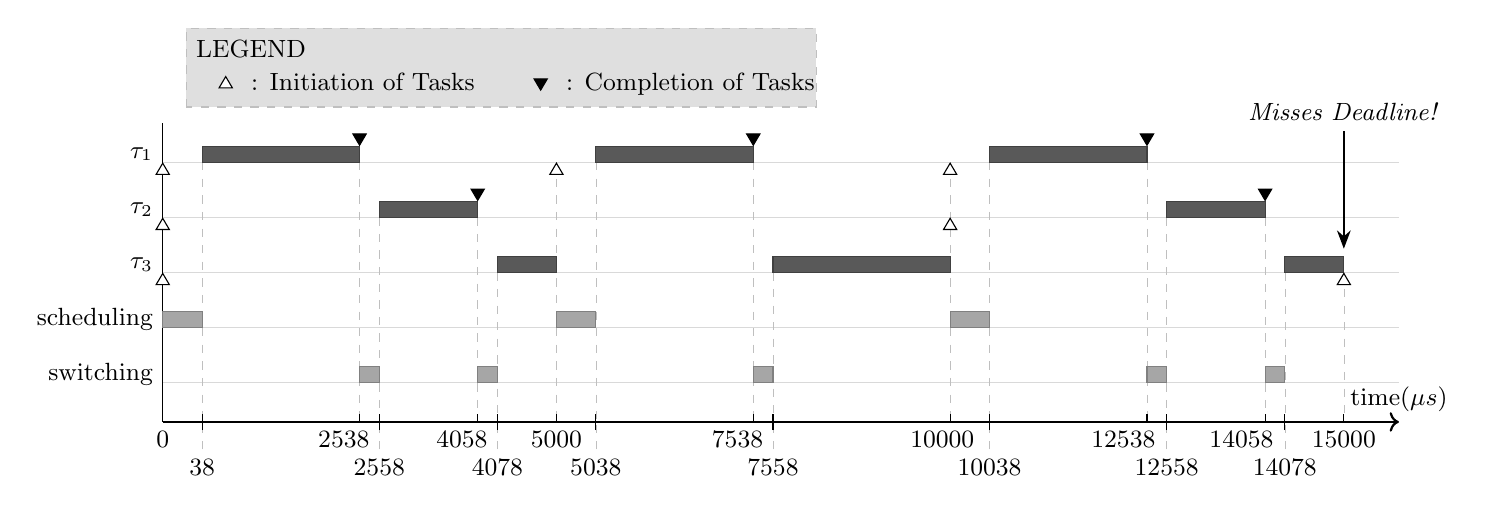
\begin{tikzpicture}[font=\small,
    % styles
    system task/.style={fill=gray!70,draw=gray},
    periodic task/.style={fill=gray!70!black,draw=gray!50!black},
    task line/.style={gray!30,very thin},
    time line/.style={gray!50,very thin,dashed},
    short line/.style={gray!50,very thin,dashed},
    init/.style={{Triangle[fill=white,scale=1.3]}-},
    complete/.style={{Triangle[scale=1.3]}-}]

  % grid
  \foreach \x in {0.5,1.2,...,3.3}
    \draw[task line] (0,\x) -- (15.7,\x);

  % time indicator
  \draw (0,0) node [below] {$0$};
  \draw[time line] (0.5,3.3) -- (0.5,0);
  \draw (0.5,-0.35) node [below] {$38$} [short line] -- +(0,0.35);
  \draw (0.5,-3pt) -- (0.5,3pt);
  \draw[time line] (2.5,3.3) -- (2.5,0);
  \draw (2.3,0) node [below] {$2538$};
  \draw (2.5,0) -- (2.5,3pt);
  \draw[time line] (2.75,2.6) -- (2.75,0);
  \draw (2.75,-0.35) node [below] {$2558$} [short line] -- +(0,0.35);
  \draw (2.75,-3pt) -- (2.75,3pt);
  \draw[time line] (4,2.6) -- (4,0);
  \draw (3.8,0) node [below] {$4058$};
  \draw (4,0) -- (4,3pt);
  \draw[time line] (4.25,1.9) -- (4.25,0);
  \draw (4.25,-0.35) node [below] {$4078$} [short line] -- +(0,0.35);
  \draw (4.25,-3pt) -- (4.25,3pt);

  \draw[time line] (5,3.3) -- (5,0);
  \draw (5,0) node [below] {$5000$};
  \draw (5,0) -- (5,3pt);
  \draw[time line] (5.5,3.3) -- (5.5,0);
  \draw (5.5,-0.35) node [below] {$5038$} [short line] -- +(0,0.35);
  \draw (5.5,-3pt) -- (5.5,3pt);
  \draw[time line] (7.5,3.3) -- (7.5,0);
  \draw (7.3,0) node [below] {$7538$};
  \draw (7.5,0) -- (7.5,3pt);
  \draw[time line] (7.75,1.9) -- (7.75,0);
  \draw (7.75,-0.35) node [below] {$7558$} [short line] -- +(0,0.35);
  \draw (7.75,-3pt) -- (7.75,3pt);

  \draw[time line] (10,3.3) -- (10,0);
  \draw (9.9,0) node [below] {$10000$};
  \draw (10,0) -- (10,3pt);
  \draw[time line] (10.5,3.3) -- (10.5,0);
  \draw (10.5,-0.35) node [below] {$10038$} [short line] -- +(0,0.35);
  \draw (10.5,-3pt) -- (10.5,3pt);
  \draw[time line] (12.5,3.3) -- (12.5,0);
  \draw (12.2,0) node [below] {$12538$};
  \draw (12.5,0) -- (12.5,3pt);
  \draw[time line] (12.75,2.6) -- (12.75,0);
  \draw (12.75,-0.35) node [below] {$12558$} [short line] -- +(0,0.35);
  \draw (12.75,-3pt) -- (12.75,3pt);
  \draw[time line] (14,2.6) -- (14,0);
  \draw (13.7,0) node [below] {$14058$};
  \draw (14,0) -- (14,3pt);
  \draw[time line] (14.25,1.9) -- (14.25,0);
  \draw (14.25,-0.35) node [below] {$14078$} [short line] -- +(0,0.35);
  \draw (14.25,-3pt) -- (14.25,3pt);
  \draw[time line] (15,1.9) -- (15,0);
  \draw (15,0) node [below] {$15000$};
  \draw (15,0) -- (15,3pt);

  % axes
  \draw[->,thick] (0,0) -- (15.7,0) node [above] {time(${\mu}s$)};
  \draw[thin] (0,0) -- (0,3.8);

  % tips of tasks
  \draw (0,0.6) node [left] {switching};
  \draw (0,1.3) node [left] {scheduling};
  \draw (0,2) node [left] {$\tau_3$};
  \draw (0,2.7) node [left] {$\tau_2$};
  \draw (0,3.4) node [left] {$\tau_1$};

  % tasks
  \filldraw[system task] (0,1.2) rectangle +(0.5,0.2);
  \filldraw[periodic task] (0.5,3.3) rectangle +(2,0.2);
  \filldraw[system task] (2.5,0.5) rectangle +(0.25,0.2);
  \filldraw[periodic task] (2.75,2.6) rectangle +(1.25,0.2);
  \filldraw[system task] (4,0.5) rectangle +(0.25,0.2);
  \filldraw[periodic task] (4.25,1.9) rectangle +(0.75,0.2);
  
  \filldraw[system task] (5,1.2) rectangle +(0.5,0.2);
  \filldraw[periodic task] (5.5,3.3) rectangle +(2,0.2);
  \filldraw[system task] (7.5,0.5) rectangle +(0.25,0.2);
  \filldraw[periodic task] (7.75,1.9) rectangle +(2.25,0.2);
  
  \filldraw[system task] (10,1.2) rectangle +(0.5,0.2);
  \filldraw[periodic task] (10.5,3.3) rectangle +(2,0.2);
  \filldraw[system task] (12.5,0.5) rectangle +(0.25,0.2);
  \filldraw[periodic task] (12.75,2.6) rectangle +(1.25,0.2);
  \filldraw[system task] (14,0.5) rectangle +(0.25,0.2);
  \filldraw[periodic task] (14.25,1.9) rectangle +(0.75,0.2);

  % initiation of tasks
  \foreach \x in {0,5,10}
    \draw [init] (\x,3.3) -- +(0,-0.1);
  \foreach \x in {0,10}
    \draw [init] (\x,2.6) -- +(0,-0.1);  
  \foreach \x in {0,15}
    \draw [init] (\x,1.9) -- +(0,-0.1); 

  % completion of tasks
  \draw [complete] (2.5,3.5) -- +(0,0.1);
  \draw [complete] (4,2.8) -- +(0,0.1);
  \draw [complete] (7.5,3.5) -- +(0,0.1);
  \draw [complete] (12.5,3.5) -- +(0,0.1);
  \draw [complete] (14,2.8) -- +(0,0.1);

  % text
  \draw[{Stealth}-,thick] (15,2.2) -- +(0,1.5)
    node [above] {\emph{Misses Deadline!}};

  % legend
  \begin{scope}[xshift = -1.2cm]  
    \draw [fill=gray!25,draw=gray!50,dashed] (1.5,4) rectangle +(8,1);
    \draw (1.5,4.5) node [above right] {LEGEND};
    \draw [init] (2,4.4) -- +(0,-0.1);
    \draw (2.2,4.55) node [below right] {: Initiation of Tasks};
    \draw [complete] (6,4.2) -- +(0,0.1);
    \draw (6.2,4.55) node [below right] {: Completion of Tasks};
  \end{scope}
\end{tikzpicture}
\caption{A counterexample of schedulability in Scenario~(iv). The first
  job instance of $\tau_3$ misses its deadline at time $15ms$, which
  is the initiation time for the second job instance of $\tau_3$.}
\label{f:counterexample}
\end{figure*}

Instantiating our model on dense time domain and choosing the
\emph{maximal time sampling strategy}, the results of the model
checking show that the correctness property holds in all scenarios. As
to the schedulability property, it holds in Scenarios~(i-iii), but
fails in Scenario~(iv).  One counterexample of the schedulability
within Scenario~(iv), returned by the model checking command, is
pictured in Figure~\ref{f:counterexample}, where the third task
$\tau_3$ misses its deadline at the time $15ms$.

The results above have demonstrated that our approach is capable of
handling realistic industrial systems. However to further exam the
efficiency of our approach, we also apply our method to larger test
scenarios. Test scenarios are generated randomly. We verify the
schedulability of them under the above setting on an Intel Core 2 Quad
Q9550, 2.83GHz, 4-cores machine with 8GB RAM running 64-bit Ubuntu
15.04. Among the 50 generated test scenarios with 5 tasks, we find
that the execution time of the model checking command for each
scenario varies from about $300ms$ up to a timeout, which is set to
$90$ minutes. This is because the efficiency of model checking depends
on the scale of the state space. And the scale is further positively
correlated with $mn$, where $m$ is the upper bound of $timer$ and $n$
is the number of periodic tasks. By the generated test scenarios, it
turns out that the model checking command for schedulability in our
model is able to handle scenarios, where $mn$ is up to about $10^6$,
in an acceptable period of time say $90$ minutes.


\hide{
\begin{figure*}[!t]
\centering
\begin{picture}(300,120)(0,-10)
\thicklines
\put(0,0){\vector(1,0){320}}
\put(305,5){time(${\mu}s$)}
\thinlines
\put(0,0){\line(0,1){110}}
\put(-25,97){task$0$}
\put(-25,77){task$1$}
\put(-25,57){task$2$}
\put(-50,37){scheduling}
\put(-45,17){switching}
\put(-2,-8){$0$}

\dashline[30]{3}(0,100)(250,100)
\dashline[30]{3}(0,80)(280,80)
\dashline[30]{3}(0,60)(300,60)
\dashline[30]{3}(0,40)(210,40)
\dashline[30]{3}(0,20)(285,20)


\dashline[30]{3}(10,-10)(10,100)
\thicklines
\textcolor{red}{\put(0,40){\line(1,0){10}}}
\put(8,-18){$9$}

\thinlines
\dashline[30]{3}(50,0)(50,100)
\thicklines
\textcolor{blue}{\put(10,100){\line(1,0){40}}}
\put(35,-8){$2509$}

\thinlines
\dashline[30]{3}(55,-10)(55,80)
\thicklines
\textcolor{red}{\put(50,20){\line(1,0){5}}}
\put(46,-18){$2513$}

\thinlines
\dashline[30]{3}(80,0)(80,80)
\thicklines
\textcolor{blue}{\put(55,80){\line(1,0){25}}}
\put(65,-8){$4013$}

\thinlines
\dashline[30]{3}(85,-10)(85,60)
\thicklines
\textcolor{red}{\put(80,20){\line(1,0){5}}}
\put(76,-18){$4017$}

\thinlines
\dashline[30]{3}(100,0)(100,60)
\thicklines
\textcolor{blue}{\put(85,60){\line(1,0){15}}}
\put(90,-8){$5000$}

\thinlines
\dashline[30]{3}(110,-10)(110,100)
\thicklines
\textcolor{red}{\put(100,40){\line(1,0){10}}}
\put(101,-18){$5009$}

\thinlines
\dashline[30]{3}(150,0)(150,100)
\thicklines
\textcolor{blue}{\put(110,100){\line(1,0){40}}}
\put(135,-8){$7509$}

\thinlines
\dashline[30]{3}(155,-10)(155,60)
\thicklines
\textcolor{red}{\put(150,20){\line(1,0){5}}}
\put(146,-18){$7513$}

\thinlines
\dashline[30]{3}(200,0)(200,60)
\thicklines
\textcolor{blue}{\put(155,60){\line(1,0){45}}}
\put(185,-8){$10000$}

\thinlines
\dashline[30]{3}(210,-10)(210,100)
\thicklines
\textcolor{red}{\put(200,40){\line(1,0){10}}}
\put(198,-18){$10009$}

\thinlines
\dashline[30]{3}(250,0)(250,100)
\thicklines
\textcolor{blue}{\put(210,100){\line(1,0){40}}}
\put(230,-8){$12509$}

\thinlines
\dashline[30]{3}(255,-10)(255,80)
\thicklines
\textcolor{red}{\put(250,20){\line(1,0){5}}}
\put(243,-18){$12513$}

\thinlines
\dashline[30]{3}(280,0)(280,80)
\thicklines
\textcolor{blue}{\put(255,80){\line(1,0){25}}}
\put(260,-8){$14013$}

\thinlines
\dashline[30]{3}(285,-10)(285,60)
\thicklines
\textcolor{red}{\put(280,20){\line(1,0){5}}}
\put(272,-18){$14017$}

\thinlines
\dashline[30]{3}(300,0)(300,60)
\thicklines
\textcolor{blue}{\put(285,60){\line(1,0){15}}}
\put(289,-8){$15000$}

\textcolor{red}{\put(300,60){\vector(-1,0){0}}}

\end{picture}
\caption{A Counterexample of Scenario (iv).}
\label{f:counterexample}
\end{figure*}
}

\subsection{Evaluation}
%\subsection{Soundness and Completeness of the Analysis}
We now show in this section that our results are both sound and
complete.

An analysis method is called \emph{sound} if any counterexample found
using such a method is a real counterexample of the question, and
\emph{complete} if the fact that no counterexample can be found using
such a method implies no counterexample exists for the question in
analysis. The soundness of our results is trivial to check, simply by
examining the counterexamples found. For instance, the counterexample
shown in Figure~\ref{f:counterexample} is a real counterexample,
implying that the result for schedulability of Scenario~(iv) is
sound. But this is not the case for completeness, since we choose
instantiating our model on dense time domain to make it more real but
giving rise to an infinite state space which is unfeasible to exhaust.

In general, completeness of untimed model checking cannot be achieved
for any systems, any time sampling strategies and any
properties. However, \"Olveczky and Meseguer proved the completeness
of untimed temporal logic model checking, under the maximal time
sampling strategy, for a large class of real-time systems possessing a
set of ``good'' properties that is called \emph{time-robustness}, and
for a set of ``good'' LTL formulae constructed by
\emph{tick-invariant} propositions\footnote{We avoid introducing the
  definitions of time-robustness and tick-invariance, due to the
  requirements of extra rewriting logic
  background.}~\cite{DBLP:journals/entcs/OlveczkyM07a}:
\begin{theorem}[\cite{DBLP:journals/entcs/OlveczkyM07a}]
\label{t:completeness}
Given a time-robust real-time rewrite theory $\cal R$, a set $AP$ of
tick-invariant atomic propositions, an LTL formula $\Phi$ (excluding
the \emph{next} operator $\bigcirc$) whose atomic propositions are
contained in $AP$. The untimed temporal logic model checking verifying
$\Phi$ is \emph{complete} under the maximal time sampling strategy.
\end{theorem}

Therefore, we achieve the following theorem, showing that the results
in Section~\ref{ss:results} are complete.
\begin{theorem}
\label{t:main}
Our approach using untimed model checking to verify the schedulability
and the correctness of our model is complete.
\end{theorem}
\begin{IEEEproof}
By showing that our model is time-robust and that the two defined
atomic propositions--\verb|taskTimeout| and \verb|correct|--are
tick-invariant, then using Theorem~\ref{t:completeness}. For a more
detailed proof, see the Appendix.
\end{IEEEproof}


\hide{
In order to prove the completeness of our verification, we need little
adjustments to our model.  For each task $\tau_i$, we collapse its
computation requirement $[C_i^{min},C_i^{max}]$ into the single value
$C_i^{max}$.  That is, in the adjusted model, we use the maximum time
that is possible to be required to complete the task, as in the
standard setting. The adjustment is reasonable for verifying our
properties, since the schedulability and correctness of the adjusted
model imply the schedulability and correctness of our original
model. In particular, this is because we can prove the followings.
\begin{lemma}
\label{l:max}
Assume $t_s, t_f$ are the times at which a job of $\tau_i$ starts and
completes its execution, respectively. Let $S_i$ be the set of tasks,
which have priorities higher than $\tau_i$ or equal to it, including
the system tasks scheduling and switching. Assumed $t_s$ is fixed,
$t_f$ reaches its maximum, if all job instances of each task
$\tau_j\in S_i$, which execute between $t_s$ and $t_f$, are completed
in time $C_j^{max}$.
\end{lemma}
\begin{IEEEproof} 
Note that each job instance that executes between $t_s$ and $t_f$
corresponds to some task in $S_i$. Assume the number of job instances
of task $\tau_j\in S_i$ is $m_j$, and they execute for time
$C_j^1,C_j^2,\ldots,C_j^{m_j}$ respectively to complete. We have
$m_i=1$. Then assume the number of interrupts between $t_s$ and $t_f$
is $m_{int}$, the corresponding $m_{int}$ scheduling stages take time
$C_{sch}^1,\ldots,C_{sch}^{m_{int}}$, respectively. By our definition
of switching, the number of switching stages between $t_s$ and $t_f$
is $M_{swi}=\Sigma_{k=1}^{i-1}m_k$, we assuming they execute for
$C_{swi}^1,\ldots,C_{swi}^{M_{swi}}$ to complete. It follows that
$t_f-t_s=\Sigma_{j=1}^i\Sigma_{k=1}^{m_j}C_j^k+\Sigma_{k=1}^{m_{int}}C_{sch}^k+\Sigma_{k=1}^{M_{swi}}C_{swi}^k$. Along
the timeline, when $C_j^k$, $C_{sch}^k$ or $C_{swi}^k$ increases,
$m_j$, $m_{int}$ and/or $M_{swi}$ may increase as well. Therefore,
$t_f$ reaches its maximum when $C_j^k$, $C_{sch}^k$ and $C_{swi}^k$
reach their maximum, hence the statement.
\end{IEEEproof}
\begin{theorem}
\label{th:max}
Given a set of tasks that is schedulable when the computation
requirement of each task $\tau_i$ equals $C_i^{max}$, this set remains
still schedulable when some job instances of some $\tau_i$ become
possible to terminate in time $t\le C_i^{max}$.
\end{theorem}
\begin{IEEEproof}
By investigating the effects on the completion time of some job
instance when reducing other job instances' computation requirements,
and using Lemma~\ref{l:max}.
\end{IEEEproof}

We achieve the same verification results in the adjusted model as in
our original one: while correctness holds within all scenarios,
schedulability holds only in Scenarios~(i-iii)\footnote{In fact,
  positive results in the original model imply positive results in the
  adjusted one, since the set of behaviors of the adjusted model is a
  subset of those of the original.} but fail in Scenario~(iv). Since
the adjusted model is time-robust and our defined atomic
propositions--\verb|taskTimeout| and \verb|correct|--are
tick-stabilizing, our analysis using untimed model checking on the
adjusted model is complete by Theorem~\ref{t:completeness}. Therefore
by Theorem~\ref{th:max}, the results shown in Section~\ref{ss:results}
for our original model are complete.
}

\hide{
To apply Theorem~\ref{t:completeness} on our analysis to show the
completeness, we only need to prove time-robustness of our model and
tick-stabilization of our defined atomic propositions,
\verb|taskTimeout| and \verb|scheduleCorrectly|. The latter is quite
trivial, while the former requires little adjustments to the model,
which collapse the possible finishing interval for some periodic task
into a single value that should be assigned to the possible maximum
computation time. Then we can apply Lemma~\ref{l:timerobustness} to
prove the time-robustness of our (adjusted) model.
\begin{lemma}
\label{l:timerobustness}
An object-oriented specification $\cal R$, with a conventional tick
rule, is \emph{time-robust} if the following conditions are satisfied
for all appropriate \emph{ground} terms $t$ and $r,r'$:

\noindent
(i) $mte(\delta(t,r))=mte(t)\dotdiv r$, for all $r\le mte(t)$;

\noindent
(ii) $\delta(t,0)=t$;

\noindent
(iii) $\delta(\delta(t,r),r')=\delta(t,r+r')$, for $r+r'\le mte(t)$;

\noindent
(iv) $mte(\sigma(l))=0$ for each ground instance $\sigma(l)$ of a
left-hand side of an instantaneous rewrite rule.
\end{lemma}

We achieve the same verification results for the adjusted model as for
the original one: schedulability and correctness hold in Scenarios
(i-iii) but fail in Scenario~(iv). The only thing remained to show the
completeness of our results is to prove the reasonability of the
adjustments, that is, if a set of tasks (including system ones) is
schedulable when the computation time of some task $\tau_i$ in it
equals to $C_i^{max}$, then when some jobs of $\tau_i$ become possible
to finish in time $r\le C_i^{max}$, the set of tasks remains still
schedulable. This is done by proving Lemma~\ref{l:max} and considering
\verb|scheduling| and \verb|switching| as having same and higher
priority than all periodic tasks.
\begin{lemma}
\label{l:max}
Assume the time $r_s$ at which a job of $\tau_i$ starts running is
fixed. The time $r_f$, at which this job finishes, reaches its maximum
if all job instances of tasks $\tau$'s, the priorities of which are
higher than or equal to that of $\tau_i$, running between $r_s$ and
$r_f$ finish in their maximum possible computation time.
\end{lemma}
}

\section{Related Work}
\label{s:relate}
In this section we discuss our results with related
work in three directions.

Considering schedulability test, Liu and
Layland~\cite{DBLP:journals/jacm/LiuL73} gave the famous sufficient
condition that a set of periodic tasks is schedulable with respect to
RMS if $\displaystyle \Sigma^n_{i=1} C_i/T_i \le n(2^{1/n}-1)$
holds. Then a more sufficient condition, known as \emph{Hyperbolic
  Bound}, which has the same complexity as Liu and Layland's, was
proposed in~\cite{DBLP:journals/tc/BiniBB03}. On the other hand,
necessary and sufficient conditions for schedulability were derived
independently in~\cite{DBLP:journals/rts/SpruntSL89}
and~\cite{audsley1993deadline}, requiring more sophisticated analysis
on the task set. Nevertheless, all these results take no overhead into
account, being not as realistic as ours. Katcher et al. did consider
overhead in their schedulability analysis, under several models based
on different kinds of popular
implementations~\cite{DBLP:journals/tse/KatcherAS93}.  However, our
target implementation is not in their scope. Furthermore, compared
with those theoretical analyses, our approach based on formal modeling
and verification has three advantages. One is that if our
schedulability test answers ``no'', it returns at the same time a real
counterexample, which is able to guide our engineer to adjust the
design, by changing either the priorities or even the scheduling
algorithm. The second is that, when a fresh scheduling strategy is
applied, our analysis can be adjusted only by modifying the model,
while theoretical approaches may need thorough analyses and reasoning.
The last one is that, considering overhead and details of hardware do
introduce some kind of non-determinism into the model. For example, in
our model, if the running task is complete \emph{right} at the time
when an interrupt request occurs, two different behaviors are
possible: (i) the system performs task switching, during which the
interrupt request is masked, hence the scheduling and initiation of
tasks may be delayed; (ii) the system answers the interrupt request
immediately, the switching being delayed. Tackling such
non-determinism via theoretical analyses seems more complicated than
our automatic approach.

\cite{TianD2011} and~\cite{DBLP:conf/iceccs/CuiDT14} also made use of
model checking to analyze the RMS algorithm along the same line but
with different languages and tools. The RMS algorithm is investigated
using an extension of SPIN~\cite{DBLP:journals/tse/Holzmann97}
in~\cite{TianD2011}, while the logic programming language
TMSVL~\cite{DBLP:conf/icfem/HanDW12} and its model checker are applied
in~\cite{DBLP:conf/iceccs/CuiDT14}. The work presented
in~\cite{TianD2011} and~\cite{DBLP:conf/iceccs/CuiDT14} has two main
differences with ours. The first one, which is also the motivational
one, is that they considered only the ideal setting of the algorithm
as in~\cite{DBLP:journals/jacm/LiuL73}, instead of an implementation
which contains much more complex details. In fact, our model of the
implementation can easily degenerate to a model of the RMS algorithm,
if we let the times for scheduling and switching be zero. The other
difference is that when adding a new task into the task set, the
models in~\cite{TianD2011} and~\cite{DBLP:conf/iceccs/CuiDT14} should
be modified by explicitly defining a sub-model of the new task and its
behaviors. In particular, the scheduling part of the model
in~\cite{TianD2011} needs adjustments as well to include a new
task. Nevertheless, a new task set is specified in our approach merely
by giving a new initial state, without necessity to modify the model,
as already emphasized in Section~\ref{ss:results}. On the other hand,
\cite{TianD2011} used a discrete time domain in the model, while we
employ a generic time domain, which is flexible to be instantiated on
either discrete or dense ones. In~\cite{DBLP:conf/iceccs/CuiDT14}, the
time domain is dense, and a modeling strategy like our maximal time
sampling strategy is applied to reduce the state space. However, a
completeness statement like Theorem~\ref{t:main} was not given
in~\cite{DBLP:conf/iceccs/CuiDT14}.

Finally, Maude and Real-Time Maude have been successfully applied on
large numbers of applications~\cite{DBLP:journals/jlp/Meseguer12},
especially on communication protocols, real-time and cyber-physical
systems. But few results are achieved on scheduling problems. RMS is
investigated using Real-Time Maude for the first time.

\section{Conclusion}
\label{s:conclusion}
We have formally modeled a realistic implementation of RMS using
Real-Time Maude, a modeling language based on rewriting logic. By
taking into account the overhead of scheduling and switching, and by
modeling some mechanism of the hardware, our model contains sufficient
details to be analyzed for the behaviors of the real target
system. Two important properties--schedulability and correctness--are
verified by model checking on our model, within several key
scenarios. We demonstrate the soundness and completeness of our
results.


\appendix[Proof of Theorem~\ref{t:main}]
\label{a:proof}
\setcounter{theorem}{0}
\renewcommand{\thetheorem}{\thesection.\arabic{theorem}}
\newcommand{\lrps}[2]{\rightarrow^{#1}_{#2}}

We show here a detailed proof of Theorem~\ref{t:main}.

Some more preliminaries from~\cite{DBLP:journals/entcs/OlveczkyM07a}
are needed. A term $t$ is called \emph{ground} if it contains no
variables. For a set $P\subseteq AP$ of atomic propositions and ground
terms $t,t'$, we write $t\simeq_P t'$ (or $t\simeq t'$ for simplicity
when $P$ is implicit) if $t$ and $t'$ satisfy exactly the same set of
propositions from $P$.

Time-robustness is a set of properties expected from a well-behaved
real-time rewrite theory. We avoid introducing the accurate definition
of time-robustness, but instead give the following lemma to prove
time-robustness:
\begin{lemma}[\cite{DBLP:journals/entcs/OlveczkyM07a}]
\label{l:timerobustness}
Let $\cal R$ be an object-oriented specification with a standard tick
rule, and let the infinity element \verb|INF| be the only element in
the time domain which is not a normal time value.
%and let the time domain be \emph{linear}.
Then $\cal R$ is time-robust if the following conditions are satisfied
for all appropriate ground terms $t$ and $r,r'$:
\begin{enumerate}
\item
[(i)] \verb|mte(delta(|$t$\verb|,|$r$\verb|))| $=$
\verb|mte(|$t$\verb|) monus |$r$, for all $r\le$
\verb|mte(|$t$\verb|)|, where \verb|monus| is the built-in minus
operation defined on sort \verb|Time|;

\item
[(ii)] \verb|delta(|$t$\verb|,|$0$\verb|)| $= t$;

\item
[(iii)] \verb|delta(delta(|$t$\verb|,|$r$\verb|),|$r'$\verb|)| $=$
\verb|delta(|$t$\verb|,|$r+r'$\verb|)|, for $r+r'\le$
\verb|mte(|$t$\verb|)|;

\item
[(iv)] \verb|mte(|$\sigma(l)$\verb|)|$= 0$ for each ground instance
$\sigma(l)$ of each left-hand side of an instantaneous rewrite rule.
\end{enumerate}
\end{lemma}

Each one-step rewrite can be categorized and then tick-invariance can
be defined:
\begin{definition}[\cite{DBLP:journals/entcs/OlveczkyM07a}]
A one-step rewrite $t\lrps{r}{1}t'$ using a tick rule and having
duration $r$ is:\\
- a \emph{maximal tick step}, written $t\lrps{r}{max}t'$, if there is
no time value $r'>r$ such that $t\lrps{r'}{1}t''$ for some $t''$; \\
- an \emph{$\infty$ tick step}, written $t\lrps{r}{\infty}t'$, if
for each time value $r'>0$, there is a tick rewrite step
$t\lrps{r'}{1}t''$; and \\
- a \emph{non-maximal tick step} if there is a maximal tick step
$t\lrps{r'}{max}t''$ for $r'>r$.
\end{definition}
\begin{definition}[\cite{DBLP:journals/entcs/OlveczkyM07a}]
  A time-robust specification $\cal R$ is \emph{tick-invariant} with
  respect to a set $P$ of propositions if and only if it is the case
  that $t\simeq_P t'$ holds for each non-maximal or $\infty$ tick step
  $t\lrps{r}{}t'$.
\end{definition}

The following lemma is needed to prove the tick-invariance of our
defined propositions:
\begin{lemma}[\cite{DBLP:journals/entcs/OlveczkyM07a}]
\label{l:tickinv}
Let $\cal R$ be a time-robust object-oriented specification with a
standard tick rule, and let the infinity element \verb|INF| be the
only element in the time domain which is not a normal time value.
%and let the time domain be \emph{linear}. 
Then $\cal R$ is tick-invariant with respect to a set $P$ of atomic
propositions if \verb|{|$t$\verb|}| $\simeq_P$
\verb|{delta(|$t$\verb|,|$r$\verb|)}| for all $t,r$ with $r<$
\verb|mte(|$t$\verb|)|.
\end{lemma}

\newcommand{\mteTask}[2]{\texttt{mteTask(}#1\texttt{,}#2\texttt{)}}
\newcommand{\deltaTask}[3]{\texttt{deltaTask(}#1\texttt{,}#2\texttt{,}#3\texttt{)}}
\newcommand{\mteIS}[1]{\texttt{mteIS(}#1\texttt{)}}
\newcommand{\deltaIS}[2]{\texttt{deltaIS(}#1\texttt{,}#2\texttt{)}}
\newcommand{\IntSrc}[3]{\texttt{<}#1\texttt{:IntSrc|val:}#2\texttt{,cycle:}#3\texttt{>}}
\newcommand{\mteIr}[1]{\texttt{mteIr(}#1\texttt{)}}
\newcommand{\mteS}[1]{\texttt{mte(}#1\texttt{)}}
\newcommand{\deltaS}[2]{\texttt{delta(}#1\texttt{,}#2\texttt{)}}
 
Several auxiliary lemmas are proved:
\begin{lemma}
\label{l:auxtask}
Given $ID$ of sort \verb|MaybeNat| and $L$ of sort \verb|TaskList|,
\verb|mteTask(|$ID$\verb|,deltaTask(|$ID$\verb|,|$L$\verb|,|$r$\verb|))|
$=$ \verb|mteTask(|$ID$\verb|,|$L$\verb|)| \verb|monus| $r$ for all
$r\le$ \verb|mteTask(|$ID$\verb|,|$L$\verb|)|.
\end{lemma}
\begin{IEEEproof}
If $ID=$ \verb|none|, the case is trivial. By definition,
\verb|mteTask(none,deltaTask(none,|$L$\verb|,|$r$\verb|))| $=$
\verb|mteTask(none,|$L$\verb|)| $=$ \verb|INF| $=$
\verb|mteTask(none,|$L$\verb|)| \verb|monus| $r$. Otherwise, $ID=$
\verb|some| $N$ with $N$ of sort \verb|Nat|. Assume that the
\verb|cnt| of the $N$th task in $L$ is
\verb|[|$r_e$\verb|/|$C$\verb|]|. Then by definition,
\verb|deltaTask(|$ID$\verb|,|$L$\verb|,|$r$\verb|)| $= L'$, where the
$N$th task in $L'$ has \verb|cnt| value being
\verb|[|$(r_e+r)$\verb|/|$C$\verb|]|. Hence,
\begin{IEEEeqnarray*}{Cl}
  & \mteTask{ID}{\deltaTask{ID}{L}{r}}
\\  
= & \mteTask{ID}{L'}
\\
= & C~\verb|monus|~(r_e+r) 
= (C~\verb|monus|~r_e)~\verb|monus|~r 
\\
= & \mteTask{ID}{L}~\verb|monus|~r~. 
\end{IEEEeqnarray*}
\end{IEEEproof}
\begin{lemma}
\label{l:auxis}
Given $ISRC$ of class \verb|IntSrc| representing an reasonable state
of interrupt source in our model, \mteIS{\deltaIS{$ISRC$}{$r$}} $=$
\mteIS{$ISRC$} \verb|monus| $r$ for all $r\le$ \mteIS{$ISRC$}.
\end{lemma}
\begin{IEEEproof}
A reasonable $ISRC$ must be of the form \IntSrc{$O$}{$v$}{$T$} with
$v\le T$. Thus by definition, 
\begin{IEEEeqnarray*}{Cl}
  & \mteIS{\deltaIS{ISRC}{r}}
\\  
= & \mteIS{\IntSrc{O}{(v~\texttt{monus}~r)}{T}}
\\
= & v~\verb|monus|~r
= \mteIS{ISRC}~\verb|monus|~r~.
\end{IEEEeqnarray*}
\end{IEEEproof}
\begin{lemma}
\label{l:auxhw}
Given $HW$ of sort \verb|Hardware|, for all $r\le$ \mteIr{$HW$},
\mteIr{$HW$} $=$ \mteIr{$HW$} \verb|monus| $r$.
\end{lemma}
\begin{IEEEproof}
  It concludes by discussing on whether there exists an interrupt
  request detected in $HW$.
\end{IEEEproof}

Now we can present the detailed proof of Theorem~\ref{t:main}:
\noindent
\begin{IEEEproof}[Proof of Theorem~\ref{t:main}]
We first prove the time-robustness of our model by
Lemma~\ref{l:timerobustness}.  Instantiated on the built-in dense time
domain \verb|POSRAT-TIME-DOMAIN-WITH-INF|, our model has \verb|INF| as
the only element which is not a normal time value. As presented in
Section~\ref{ss:timedbehavior}, only a single standard tick rule is
defined. Hence our model is time-robust by
Lemma~\ref{l:timerobustness} provided conditions (i-iv) hold.

Condition~(i). We must prove \verb|mte(delta(|$s$\verb|,|$r$\verb|))|
$=$ \verb|mte(|$s$\verb|)| \verb|monus| $r$ for all $r\le$
\verb|mte(|$s$\verb|)|, with $s$ being a system state of sort
\verb|System|. Let $s$ be of the form
$(\mathit{L}~\mathit{T}~\mathit{STS}~\mathit{HW}~\mathit{ISRC})$ and
$\mathit{ID}=\verb|(|\mathit{HW}\verb|).getPc|$. We only consider the
case $\mathit{ID}$\verb|::MaybeNat| in detail, while the other case
$\mathit{ID}$\verb|::Oid| is similar. By definitions of \verb|mte| and
\verb|delta|,
\begin{IEEEeqnarray*}{Cl}
  & \mteS{\deltaS{s}{r}}
\\  
= & \mteS{\deltaTask{ID}{L}{r}
\\
  & \;\;\;\;\;\;\;\;\;T~STS~HW~\deltaIS{ISRC}{r}}
\\
= & \verb|minimum(|\mteTask{ID}{\deltaTask{ID}{L}{r}}\verb|,|
\\
  & \verb|        |\mteIS{\deltaIS{ISRC}{r}}\verb|,|
\\
  & \verb|        |\mteIr{HW}\verb|)|~.
\end{IEEEeqnarray*}
By Lemmas~\ref{l:auxtask},~\ref{l:auxis} and~\ref{l:auxhw}, it can be
further reduced:
\begin{IEEEeqnarray*}{Cl}
  & \mteS{\deltaS{s}{r}}
\\  
= & \verb|minimum(|\mteTask{ID}{L}~\verb|monus|~r~\verb|,|
\\
  & \verb|        |\mteIS{ISRC}~\verb|monus|~r~\verb|,|
\\
  & \verb|        |\mteIr{HW}~\verb|monus|~r~\verb|)|
\\
= & \verb|minimum(|\mteTask{ID}{L}\verb|,|
\\
  & \verb|        |\mteIS{ISRC}\verb|,|
\\
  & \verb|        |\mteIr{HW}\verb|)|~\verb|monus|~r
\\
= & \mteS{s}~\verb|monus|~r~.
\end{IEEEeqnarray*}

Condition~(ii) follows from the fact that $r+0=r$ and
$r$~\verb|monus|~$0=r$ for all $r$.

Condition~(iii). We must prove \deltaS{\deltaS{$s$}{$r$}}{$r'$} $=$
\deltaS{$s$}{$r+r'$} for all $r+r'\le$ \mteS{$s$}, with $s$ being a
system state of sort \verb|System|. Using the same notations as in~(i),
we only consider the case $\mathit{ID}$\verb|::MaybeNat| in detail. 
By definition, the left side of the equation
\begin{IEEEeqnarray*}{Cl}
  & \deltaS{\deltaS{s}{r}}{r'}
\\  
= & \verb|(|\deltaTask{ID}{\deltaTask{ID}{L}{r}}{r'}
\\
  & \verb| |~T~STS~HW~\deltaIS{\deltaIS{ISRC}{r}}{r'}\verb|)|~\mbox{,}
\end{IEEEeqnarray*}
and the right side of the equation
\begin{IEEEeqnarray*}{Cl}
  & \deltaS{s}{r+r'}
\\  
= & \verb|(|\deltaTask{ID}{L}{r+r'}
\\
  & \verb| |~T~STS~HW~\deltaIS{ISRC}{r+r'}\verb|)|~\mbox{.}
\end{IEEEeqnarray*}
\deltaTask{$ID$}{\deltaTask{$ID$}{$L$}{$r$}}{$r'$} $=$
\deltaTask{$ID$}{$L$}{$r+r'$} holds by the associativity of $+$, while
\deltaIS{\deltaIS{$ISRC$}{$r$}}{$r'$} $=$ \deltaIS{$ISRC$}{$r+r'$}
holds since $(v$ \verb|monus| $r)$ \verb|monus| $r'$ $=$ $v$
\verb|monus| $(r+r')$ with $v$ of sort \verb|Time|. Thus
condition~(iii) holds.

Condition~(iv). We show that \verb|mte| of each instance of the
left-hand side of any instantaneous rule is $0$. For example,
considering the (conditional) rule \verb|interrupt-request|, with its
condition \verb|(|$ISRC$\verb|).timeout|, we know that the \verb|val|
of $ISRC$ equals $0$. Therefore,
\begin{IEEEeqnarray*}{Cl}
  & \mteS{L~T~STS~HW~ISRC}
\\  
= & \verb|minimum(|\mteTask{ID}{L}\verb|,|
\\
  & \verb|        |\mteIS{ISRC}\verb|,| \mteIr{HW}\verb|)|
\\
= & \verb|minimum(|\mteTask{ID}{L}\verb|,|~0~\verb|,| \mteIr{HW}\verb|)|
\\
= & 0~\mbox{.}
\end{IEEEeqnarray*}
The other rules can be similarly proved with their conditions. Hence
our model is time-robust by Lemma~\ref{l:timerobustness}.

Finally we prove the tick-invariance of the propositions used to
analyze our model, i.e. \verb|taskTimeout| and \verb|correct|. By
Lemma~\ref{l:tickinv}, we must prove
$\verb|{|s\verb|}|\simeq_P\verb|{|\deltaS{s}{r}\verb|}|$ with $s$ of
sort \verb|System| and $r<\mteS{s}$, that is, applying a tick rule
advancing $r$ time units will not change the value of each
proposition. Let $s$ be
$(\mathit{L}~\mathit{T}~\mathit{STS}~\mathit{HW}~\mathit{ISRC})$ and
$\verb|(|\mathit{HW}\verb|).getPc|=\mathit{ID}$.
\begin{itemize}
\item \verb|taskTimeout| holds if and only if $L$ contains an
  \verb|error|. Since \verb|delta| does not produce or eliminate
  \verb|error| in $L$, \verb|taskTimeout| holds in $s$ if and only if
  \verb|taskTimeout| holds in $\deltaS{s}{r}$ for any $r<\mteS{s}$,
  which means that our model is tick-invariant with respect to
  \verb|taskTimeout|.
\hide{ 
In our model, an \verb|error| cannot be eliminated by any operations,
hence, if \verb|taskTimeout| holds in $s$, it must hold in
$\deltaS{s}{r}$. On the other hand, \verb|error| can pop up only when
operation \verb|update_with_| is applied, i.e., only when the
instantaneous rule \verb|interrupt-handle| applies. If
\verb|taskTimeout| does not hold in $s$, it will not hold either in
$\deltaS{s}{r}$ for any $r<\mteS{s}$, since instantaneous rules cannot
apply in $\deltaS{s}{r'}$ for any $r'<\mteS{s}$ by time-robustness.}
\item The value of \verb|correct| depends on $ID$ and the status of
  each task in $L$. Similarly, \verb|delta| does not change $ID$ or
  the status of any task in $L$, hence \verb|correct| holds in $s$ if
  and only if \verb|correct| holds in $\deltaS{s}{r}$ for any
  $r<\mteS{s}$. It concludes the tick-invariance of \verb|correct|.
\end{itemize}

Therefore, by Theorem~\ref{t:completeness}, our approach using untimed
model checking to verify the schedulability and the correctness is
complete.
\end{IEEEproof}


\hide{
% use section* for acknowledgment
\ifCLASSOPTIONcompsoc
  % The Computer Society usually uses the plural form
  \section*{Acknowledgments}
\else
  % regular IEEE prefers the singular form
  \section*{Acknowledgment}
\fi

The authors would like to thank...
}

% Can use something like this to put references on a page
% by themselves when using endfloat and the captionsoff option.
\ifCLASSOPTIONcaptionsoff
  \newpage
\fi



% trigger a \newpage just before the given reference
% number - used to balance the columns on the last page
% adjust value as needed - may need to be readjusted if
% the document is modified later
%\IEEEtriggeratref{8}
% The "triggered" command can be changed if desired:
%\IEEEtriggercmd{\enlargethispage{-5in}}

% references section

% can use a bibliography generated by BibTeX as a .bbl file
% BibTeX documentation can be easily obtained at:
% http://www.ctan.org/tex-archive/biblio/bibtex/contrib/doc/
% The IEEEtran BibTeX style support page is at:
% http://www.michaelshell.org/tex/ieeetran/bibtex/
\bibliographystyle{IEEEtran}
% argument is your BibTeX string definitions and bibliography database(s)
\bibliography{IEEEabrv,submission}
%
% <OR> manually copy in the resultant .bbl file
% set second argument of \begin to the number of references
% (used to reserve space for the reference number labels box)


% biography section
% 
% If you have an EPS/PDF photo (graphicx package needed) extra braces are
% needed around the contents of the optional argument to biography to prevent
% the LaTeX parser from getting confused when it sees the complicated
% \includegraphics command within an optional argument. (You could create
% your own custom macro containing the \includegraphics command to make things
% simpler here.)
%\begin{IEEEbiography}[{\includegraphics[width=1in,height=1.25in,clip,keepaspectratio]{mshell}}]{Michael Shell}
% or if you just want to reserve a space for a photo:




\hide{

\begin{IEEEbiography}{Jiaxiang Liu}
Biography text here.
\end{IEEEbiography}


% if you will not have a photo at all:
\begin{IEEEbiographynophoto}{John Doe}
Biography text here.
\end{IEEEbiographynophoto}

% insert where needed to balance the two columns on the last page with
% biographies
%\newpage

\begin{IEEEbiographynophoto}{Jane Doe}
Biography text here.
\end{IEEEbiographynophoto}
}

% You can push biographies down or up by placing
% a \vfill before or after them. The appropriate
% use of \vfill depends on what kind of text is
% on the last page and whether or not the columns
% are being equalized.

%\vfill

% Can be used to pull up biographies so that the bottom of the last one
% is flush with the other column.
%\enlargethispage{-5in}



% that's all folks
\end{document}


